\documentclass[12pt]{report}

\usepackage[latin1]{inputenc}
\usepackage[Glenn]{fncychap}
\usepackage{graphicx}
\usepackage{tikz}
\usepackage[hidelinks]{hyperref}
\usepackage{float}
\usepackage{mathtools}
\usepackage[toc,page]{appendix}
\usepackage{amssymb}
\usepackage{tabularx}
\usepackage{longtable}
\usepackage{ifthen}	
%\usepackage{cite}

\newcommand{\argmax}[1]{\underset{#1}{\operatorname{arg}\,\operatorname{max}}\;}
\newcommand{\argmin}[1]{\underset{#1}{\operatorname{arg}
\,\operatorname{min}}\;}

%Figures aliases
%Usage: \image{path}{width}{caption}{label}
%Try to allways use \image and let latex fix positioning of figures.
%By passing 'null' as width the latex will use the figures default size
%Do however but the command at the wanted position within the text, 
%if we at a later stage want to fix the positioning of all images it could be done by rewriting this alias.
\newcommand{\image}[4]{
	\ifthenelse{\equal{false}{true}}{%true - true => latex fixes positioning, mismatch => forced positioning by float
		\begin{figure}[ht]
			\centering
			\insertImage{#1}{#2}
			\caption{#3}
			\label{#4}
		\end{figure}
	}{
		\imageHere{#1}{#2}{#3}{#4}
	}	
}
\newcommand{\imageHere}[4]{
	\begin{figure}[H]
		\centering
		\insertImage{#1}{#2}
		\caption{#3}
		\label{#4}
	\end{figure}
}
%Helper function, do not use
\newcommand{\insertImage}[2]{
	\ifthenelse{\equal{#2}{null}}{
		\includegraphics{#1}
	}{
		\includegraphics[width=#2]{#1}
	}
}
\newcommand{\wrap}[2]{
	\ifthenelse{\equal{#2}{}}{
		\begin{minipage}[t]{0.7\columnwidth}
			#1
		\end{minipage}
	}{
		\begin{minipage}[t]{#2\columnwidth}
			Backup #1
		\end{minipage}
	}
}
\newcommand{\chirp}[0]{ChIRP}

%%Force correct display style for math environments
\everymath{\displaystyle}

\begin{document}

%\begin{titlepage}
	\noindent {\large \textbf{\thesisAuthor}}
	\vspace{2cm}

	\noindent {\Huge \thesisTitle}
	\vspace{2cm}
	
	\noindent \thesisType, \thesisDate 
	\vspace{2cm}

	\noindent Artificial Intelligence Group\\ Department of Computer and Information Science\\ Faculty of Information Technology, Mathematics and Electrical Engineering\\

	\vfill
	\begin{center}
		
\includegraphics[width=3cm]{images/NTNUlogo.pdf}
	\end{center}
\end{titlepage}

%\thispagestyle{empty}
%\mbox{}\\[6pc]
%\begin{center}
%	\Large{TDT4501 Datateknikk, Master thesis}\\
%	\large{Spring 2014}\\[4pc]
%	\Huge{Educational Robotics}\\[2pc]
%	
%	\Large{Jan Tore St�lsvik}\\[1pc]
%	\Large{Nicklas Utgaard}\\[4pc]
%	%\Large{\today}\\[2pc]
	
	%PROJECT THESIS\\
%	Department of Computer Science,\\
%	NTNU, Trondheim\\[6pc]
	
%	\today
%\end{center}
%\vfill

%\noindent Supervisor 1: Pauline Haddow

%\noindent Supervisor 2: Guttorm Sindre
\setcounter{page}{0}
\pagenumbering{roman}
\section*{Abstract}
In the later years robotics has seen a huge increase within domestic use, and have now become an affordable tool in the daily life of most people.
The goal of this project was to investigate the differences between a physical and virtual robot in terms of increased content knowledge, learning motivation, and interest in science, technology, engineering and mathematics (STEM).
	%The goal of this thesis is to look into how robotics can be combined with the early education of children in K-12, in order to increase content knowledge, motivate learning and generate more interest within the STEM fields.
To investigate this we conducted an experiment at Trondheim'm International School (THIS), using a quasi-experimental setup with two treatment group, virtual and physical robot. 
	%To investigate the applicability of robotics an experiment was conducted at Trondheim's International School (THIS) 
The results showed that there does not exist a statistically significant difference in content knowledge gain, motivation or interest between the robotics group and the simulator group. 

\newpage
\section*{Sammendrag}
 De siste årene har roboter økt i popularitet innenfor vanlige hushold, og har kommet ned på ett prisnivå som gjør robotene tilgjengelig for folk flest.
Målet med denne oppgaven var å undersøke forskjellene mellom en fysisk og virtuell robot med tanke på å øke kunnskapsnivået, motivasjonen og interessen for vitenskap, teknologi, ingeniørskap og matematikk (STEM).
For å undersøke dette utførte we ett eksperiment hos Trondheim's International School (THIS), hvor vi brukte ett kvasieksperimentelt oppsett med to behandlingsgrupper, virtuell og fysisk robot.
Resultatene viste at det ikke fantes noen statistisk signifikant forskjell i økning av kunnskapsnivå, motivasjon eller interesse mellom robot gruppen og simulator gruppen.
\section*{Preface}
	This pre-master's project was carried out within the Information Management (IF) 
	group under the Department of Computer and Information Sciene (IDI) 
	at the Norwegian University of Science and Technology (NTNU)\\[1pc]
	
	Trondheim, \today\\[1pc]
	
	
	\noindent Jan Tore St�lsvik\\
	Nicklas S�rlie Utgaard
\pagenumbering{gobble}
\tableofcontents
\newpage
\listoftables
\newpage
\listoffigures
\newpage
\setcounter{page}{0}
\pagenumbering{arabic}
%\section{Literature study}
All the papers we have included have a pre post test.

Use constructionism as the theoretical base for designing robotics activities for educational purposes.

Almost all the papers say they use paperts theories in their experiements. However they only look at the experimental design of curriculum when they say that. In previous work some mention that papert talks about mental models and learning about learning. But this is never tested for. The pre post tests are merely on knowledge gains. 

They all create their own curriculum without consulting pedagogs or teacher in doing so. There is no effort to adapt it to traditional or the schools curriculum thus making it hard to say anything about applicability in schools. 

Most results are good, but the approaches are not realistic. It is hard to change the entire school system at once, and even though experimental design seems to be the most promising much other research say that math needs to be more explicitly connected to the curriculum.

We will look at how a robot can be integrated into the school. We will talk to teachers and find the best approach. We will only look at angles and turn measurement. We will focus on the robot as a mental model and ask questions that can answer whether or not a robot is better than a simulator.

\section{Pedagogic Theory}
Constructivism is not a pedagogy but a theory describing how learning happens. The theory suggests that we construct knowledge out of experiences. 
Constructionism is a pedagogy describing how to use objects to create mental models. From constructivist theories of psychology we take a view of learning as a reconstruction rather than as a transmission of knowledge. Then we extend the idea of manipulative materials to the idea that learning is most effective when part of an activity the learner experiences as constructing is a meaningful product. 

Constructivism, a model of children as builders of their own intellectual structures from jean piaget is the base constructionism is built upon. It basically says that humans generate knowledge and meaning from an interaction between their experiences and their ideas in a process called assimilation. When we assimilate we incorporate the new experience into an already existing framework without changing that framework. 

The main difference is that where piaget would explain the slower development of a particular concept by its greater complexity or formality, papert see the critical factor as the relative poverty of the culture in those materials that would make the concept concrete and simple. Aka a huge focus on objects as catalysts for knowledge.

constructivists seem to be having difficulties defining testable learning theories.

Constructionism

Chapter 1 paragrapf 2:
This powerful image of child as epistemologist caught my imagination while I was working with Piaget. In 1964, after five years at Piaget�s Center for genetic epistemology in geneva, I came away impressed by his way of looking at children as the active builders of their own intellectual structures. But to say that intellectual structures are built by the learner rather than taught by a teacher does not mean that they are built from nothing. On the contrary: Like other builders, children appropriate to their own use materials they find about them, most saliently the models and methaphores suggested by the surrounding culture. 

Teaching "at" students is replaced by assisting them to understand. Computer aided learning usually means making the computers teach the child, the computer programs the child. In paperts vision the child programs the computer and in doing so aquires a scence of mastery over a modern powerful technology.

Intelectual model building

Children learn mathematics as a living language by learning to �talk� to a computer.

Things that are seen as too formal or too mathematical will be learned just as easy in a computer rich world. Kind of disproved i guess I should read up on this in future research by papert!

Learn much as we speak instead of learning it in school.

Book is really about how a culture, a way of thinking, an idea comes to inhabit a young mind.

Learn to learn and love math

�object to think with� - turtle/robot

Learn to use touch sensors to avoid objects. 

Learning how to exercice controll over an exceptionally rich and sophisticated �micro-world� in all different cases of stuff.

Want the child to program the computer, not the computer to program the child. This to explore how themselves think.

of course the turtle can help in the teaching of traditional curriculum, but I have thought of it as a vehicle for piagetian learning, which to me is learning without curriculum.

Teaching without curriculum does not mean anarchy. It means supporting children as they build their own intellectual structures with materials drawn from the surrounding culture. 

Turtle is only one example. Use anything!

What we draw from constructivism

First off we use logo. So pretty much everything from that relates to us

Mircoworlds

We do not concern ourselves with school curriculum but we want to create a platform for teaching with a robot and as such might introduce or propose small alterations to the classroom dynamic. As papert mentions it is important for students to reach a goal by themselves, and not be programmed by the curriculum.

We will make students walk and turn according to what they think the program will do. Maybe with one arm held out in the direction they started turning and then one arm in front of them as they turn.

Notes irrelevant for our study 
Mathphobia, only have problem with things recognized as math.
School math teaching is poision and creates mathphobia

\section{Our approach}
We will use the basic ideas presented by papert.

Research shows that robots create better results, and a lot of the research is based on papert. However none explicitly mentions the reason for learning being a stronger mental model and an easier time to imagine the robot instead of alternatives. 

We would like to test our belief that using robots can ease the creation of mental models and assist in intellectual model building. In addition it is shown to be more fun and foster collaboration.

Following paperts ideas we will not be teaching students by �programming� them. Instead of using the robot as a task giver we will want them to solve tasks by programming it themselves and learn. The main difference being traditional computer systems give students tasks to complete, here the robot is merely a slave and only obeys commands.

Research done by silk again and again shows that the math needs to be made explicit when working with robots, to avoid a big focus on trial and error by students. This is also shown in many logo papers. clements work, mainly Development of turn and turn measurement concepts in a computer-based instructional unit. also mentions that trial and error and misconceptions were a big issue. For example in silks work students just try to adapt one step at a time instead of understanding underlying math. In clements case studens turned a random direciton of left or right when creating a square. If they turned the wrong way they just moved backwards instead of forward. 

The students will learn how to exercise control over a �micro-world� namely the robot through the tablet app. We will use the robot as our microworld and compare it to a simulated microworld.

We want the child to program the computer to explore how themselves think. To highlight how the students think they will perform the actions they think the robot will do before trying to run the app. By for example extending one arm turning 

Of course the turtle can help in the teaching of traditional curriculum, but I have thought of it as a vehicle for piagetian learning, which to me is learning without curriculum. We will work around the existing curriculum found at THIS.

In addition to the pedagogic believes the research largely shows that robots are fun, motivating and fosters collaboration. We will have the students working in groups of three based on the experience of the teachers at THIS.

%\chapter{PrePostTest}
\usetikzlibrary{quotes,angles,calc}
Which angle is bigger in each pair?

\begin{tikzpicture}[thick, scale= 2]
	\draw (0,0) -- (0:1);
	\draw (0,0) -- (80:1);
	\begin{scope}[shift={(2,0)}]
		\draw (0,0) -- (60:2);
		\draw (0,0) -- (20:2);
  \end{scope}
\end{tikzpicture}

\bigskip

\begin{tikzpicture}[thick, scale= 2]
	\draw (0,0) -- (45:1);
	\draw (0,0) -- (-45:1);
	\begin{scope}[shift={(2,0)}]
		\draw (0,0) -- (-45:1);
		\draw (0,0) -- (-135:1);
  \end{scope}
\end{tikzpicture}

\begin{tikzpicture}[thick, scale= 2]
	\draw (0,0) -- (60:1);
	\draw (0,0) -- (80:1);
	\begin{scope}[shift={(2,0)}]
		\draw (0,0) -- (40:1);
		\draw (0,0) -- (10:1);
  \end{scope}
\end{tikzpicture}

Find the missing measures of the angles (59 logo and geometry)

\begin{tikzpicture}
  \draw
  (3,-1) coordinate (a) node[right] {a}
  -- (0,0) coordinate (b) node[left] {b}
  -- (2,2) coordinate (c) node[above right] {c}
  pic["$\alpha$",draw=orange,<->,angle eccentricity=1.2,angle radius=1cm] {angle=a--b--c};
\end{tikzpicture}

\newcommand{\tikzAngleOfLine}{\tikz@AngleOfLine}                               
  \def\tikz@AngleOfLine(#1)(#2)#3{%                                            
  \pgfmathanglebetweenpoints{%                                                 
    \pgfpointanchor{#1}{center}}{%                                             
    \pgfpointanchor{#2}{center}}                                               
  \pgfmathsetmacro{#3}{\pgfmathresult}%                                        
  }                                                                            
\newcommand{\tikzMarkAngle}[3]{                                                
\tikzAngleOfLine#1#2{\AngleStart}                                              
\tikzAngleOfLine#1#3{\AngleEnd}                                                
\draw #1+(\AngleStart:0.15cm) arc (\AngleStart:\AngleEnd:0.15cm);              
}                                                                              

\begin{tikzpicture}[scale=4,line width=1pt]                                    
  \coordinate (A) at (0,0);                                                    
  \coordinate (B) at ($(A)+(90:1)$);                                                    
  \coordinate (C) at ($(B)+(-30:2)$);                                                
  \draw (A) -- (B) -- (C) -- cycle;                                            
	
  \tikzMarkAngle{(C)}{(B)}{(A)}   
	\node at ($(C)+(160:0.23)$) {?=\underline{\hspace{1cm}}};
	
	\tikzMarkAngle{(A)}{(B)}{(C)}
	\node at ($(A)+(45:0.23)$) {$90^\circ$};
	
	\tikzMarkAngle{(B)}{(A)}{(C)}           
	\node at ($(B)+(-60:0.23)$) {$60^\circ$};
\end{tikzpicture}  

\begin{tikzpicture}[scale=4,line width=1pt]                                    
  \coordinate (A) at (0,0);                                                    
  \coordinate (B) at ($(A)+(80:1)$);                                                    
  \coordinate (D) at ($(A)+(0:3)$);                                                
	\coordinate (C) at ($(D)+(100:1.5)$);
  \draw (A) -- (B) -- (C) -- (D) -- cycle;                                            
	
  \tikzMarkAngle{(A)}{(B)}{(D)}   
	
	\tikzMarkAngle{(C)}{(B)}{(D)}           
	
	\tikzMarkAngle{(D)}{(A)}{(C)}          
	
	\draw[shift={(B)}] (-100:0.15cm) arc (-100:10:0.15cm);
\end{tikzpicture}  

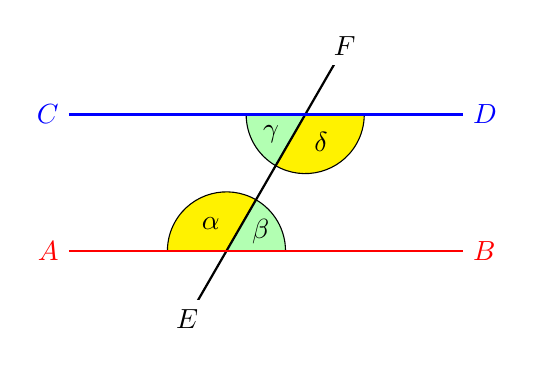
\begin{tikzpicture}
  \draw[fill=yellow] (0,0) -- (60:.75cm) arc (60:180:.75cm);
  \draw(120:0.4cm) node {$\alpha$};

  \draw[fill=green!30] (0,0) -- (right:.75cm) arc (0:60:.75cm);
  \draw(30:0.5cm) node {$\beta$};

  \begin{scope}[shift={(60:2cm)}]
    \draw[fill=green!30] (0,0) -- (180:.75cm) arc (180:240:.75cm);
    \draw (30:-0.5cm) node {$\gamma$};

    \draw[fill=yellow] (0,0) -- (240:.75cm) arc (240:360:.75cm);
    \draw (-60:0.4cm) node {$\delta$};
  \end{scope}

  \begin{scope}[thick]
    \draw (60:-1cm) node[fill=white] {$E$} -- (60:3cm) node[fill=white] {$F$};
    \draw[red]                   (-2,0) node[left] {$A$} -- (3,0) 
                                        node[right]{$B$};
    \draw[blue,shift={(60:2cm)}] (-3,0) node[left] {$C$} -- (2,0) 
                                        node[right]{$D$};
  \end{scope}
\end{tikzpicture}

Estimate the angles

\begin{tikzpicture}[scale=4,line width=1pt]                                    
  \coordinate (A) at (0,0);                                                    
  \coordinate (B) at ($(A)+(90:1)$);                                                    
  \coordinate (C) at ($(A)+(30:1)$);                                                
  \draw (A) -- (B);                                            
	\draw (A) -- (C);                                            
  \tikzMarkAngle{(A)}{(B)}{(C)}   
\end{tikzpicture}  

\begin{tikzpicture}[scale=4,line width=1pt]                                    
  \coordinate (A) at (0,0);                                                    
  \coordinate (B) at ($(A)+(90:1)$);                                                    
  \coordinate (C) at ($(A)+(0:1)$);                                                
  \draw (A) -- (B);                                            
	\draw (A) -- (C);                                            
  \tikzMarkAngle{(A)}{(B)}{(C)}   
\end{tikzpicture}  

\begin{tikzpicture}[scale=4,line width=1pt]                                    
  \coordinate (A) at (0,0);                                                    
  \coordinate (B) at ($(A)+(120:1)$);                                                    
  \coordinate (C) at ($(A)+(0:1)$);                                                
  \draw (A) -- (B);                                            
	\draw (A) -- (C);                                            
  \tikzMarkAngle{(A)}{(B)}{(C)}   
\end{tikzpicture}  

\begin{tikzpicture}[scale=4,line width=1pt]                                    
  \coordinate (A) at (0,0);                                                    
  \coordinate (B) at ($(A)+(-90:1)$);                                                    
  \coordinate (C) at ($(A)+(-135:1)$);                                                
  \draw (A) -- (B);                                            
	\draw (A) -- (C);                                            
  \tikzMarkAngle{(A)}{(B)}{(C)}   
\end{tikzpicture}  

\begin{tikzpicture}[scale=4,line width=1pt]                                    
  \coordinate (A) at (0,0);                                                    
  \coordinate (B) at ($(A)+(0:1)$);                                                    
  \coordinate (C) at ($(A)+(180:1)$);                                                
  \draw (A) -- (B);                                            
	\draw (A) -- (C);                                            
  \tikzMarkAngle{(A)}{(B)}{(C)}   
\end{tikzpicture}  

%parallelogram
\begin{tikzpicture}[scale=4,line width=1pt]                                    
  \coordinate (A) at (0,0);                                                    
  \coordinate (B) at (2,0);                                                    
  \coordinate (C) at ($(B)+(150:1)$);                                                
	\coordinate (D) at ($(A)+(150:1)$);                                                
  \draw (A) -- (B) -- (C) -- (D) -- cycle;                                            
	
  \tikzMarkAngle{(A)}{(B)}{(D)}   
	
	\tikzMarkAngle{(B)}{(A)}{(C)}
	
	\tikzMarkAngle{(C)}{(B)}{(D)}           
	\draw[shift={(D)}] (-30:0.15cm) arc (-30:0:0.15cm);      
\end{tikzpicture}  
\part{Introduction}
\chapter{Introduction}
Schools have problems with keeping students engaged and motivated courses related to science, and especially in mathematics. 
Norwegian students also perform poorly compared the students in the neighbouring countries in these courses~\cite{OECDPISA}.
%They also perform poorly to a large extent. 
Since the robotics business is growing all the time and educational robotics has been shown to have great promise we focus this project on an investigation into the potential of robotics in schools and make an effort to expand the \chirp team's horizon into the world of education. This thesis serves as an introduction into the educational world for the \chirp team at IDI. A lot of groundwork therefore had to be done in order to carry out this experiment, and we've focused on making the project applicable for future work.

\bigskip\noindent
A lot of research has been done to show that robotics can be beneficial in an educational setting.
Many researchers rely on the early work conducted by Seymour Papert within educational robotics, but often fail to fail to explain how Papert's theories are applied within their own research. 
%Many mention Papert, but fail to explain how their approach relates to his theories of learning.
%They merely state that Papert was an influence or that they use experimental design inspired by Papert's work. %, but this is only a small part of Papert's vision. 
Another common sight while reading about educational robotics is lack of research regarding the usefulness of a physical robots in itself, as it seems like most people made the jump from tradional teaching to teaching with a robot in one big jump. 
While still basing our approach on Papert's theories of mental model building, we will try to fill some of these holes. We want to test whether relatability and knowledge gains can be improved by using a physical robot compared to using a simulator confined to a local device. 

\bigskip\noindent
What we are doing is the first thesis in this area for the \chirp team. We are breaking new ground for the team, establishing collaborations and hopefully providing the basis for future work. 
Because of this we've designed our system implementation in such a way that others can expand upon it. 
%What we have implemented is designed in a way for other students to expand on. We are taking the first step. It is always the hardest. 
%There is also help in the literature but limited in this area. 

\bigskip\noindent
All we have done leads up to a pilot test at the Trondheim International School (THIS), where we tested our hypothesis and how well suited the \chirp robot was in an educational setting. 

\bigskip\noindent
The contact established between the \chirp team and the school will hopefully help foster further research within educational robotics from the \chirp team.
%We successfully created contact with them and will hopefully create a cooperation with the ChIRP group for future research. 

%\section{Context} %"'Yeah, I changed the name of this"' - Nicklas


	

\section{Motivation}
The majority of research into educational robotics shows that gains in content knowledge can be achieved using robotics. 
%Robotics are proven to be good and sometimes bad. 
However the benefits of a robot in education discussed in several papers often limit themselves to only talking about superficial aspects like fun, engagement, motivation and cooperation. 
%We want to take a closer look at why, and one of the major issues identified during a literature review was the lack of research into simulated environments. 
We want to take a closer look into the pedagogic aspects of mental model building (intellectual model building) and investigate the differences in using a physical robot compared to a simulator which is significantly cheaper to develop, buy and maintain.% a robot is better (if that is the case) than for example a simulator which is significantly cheaper to develop, buy and maintain. 

\bigskip\noindent
We find that besides mental model building which might be improved by using robots the learning experience will most definitely be new and interesting. We see this as an important aspect of the robotics experience, and therefore aim to augment our investigation to include questions that probe for attitude changes. 

%\bigskip\noindent
%Present our literature study findings. Should literature study come before the task itself?
%Nah, blir ikke det feil?

\section{Project Goals}
The goal of this project is to investigate the use of robotics in schools for the ChIRP group. We will implement an intuitive way to control the robot with a solid foundation in pedagogic theory, make necessary alterations to the ChIRP and test our assumptions on school children. There will not be enough time to fully test this system but it will serve as a platform for others to expand on in the future. 

We will also try to document our design choices and break down the pedagogic theories and relating work through a literature study to support our choices and claims to create a solid platform. 

We wish to contribute to the discussion of educational robotics both through our software implementations but also the conclusions we draw on robot vs simulator. In this way we intend to further the research in this area. 

\section{Report Structure}
This report is split into six chapters before including a set of appendices for any information which may be relevant to the reader.

\bigskip\noindent
\textbf{Chapter~\ref{part:introduction}} will provide a short introduction to the project, including motivation behind conduction the project, reseach question and the different phases of the project.

\bigskip\noindent
\textbf{Chapter~\ref{part:literature}} is dedicated to the literature review and process of conducting the literature review. 
%will the pedagogical theories used throughout the project, the process of doing the literature review, and the current state of the art for educational robotics. 

\bigskip\noindent
\textbf{Chapter~\ref{part:development}} presents our design principles and a discussion related to other software solution, before presenting the system created during this project. 

\bigskip\noindent
\textbf{Chapter~\ref{part:method}} presents our experimental setup, the procedures used, and a discussion around the reliability and validity of the study.

\bigskip\noindent
\textbf{Chapter~\ref{part:results}} provides an overview of all the results and analyses from the experiment.

\bigskip\noindent
\textbf{Chapter~\ref{part:discussion}} is the culmination of this report, and presents a discussion of the whole project before presenting our conclusion and proposals for future work. 



\part{Research Approach}
\chapter{Approach}
\chapter{Research questions}
We have found a couple of research questions through an initial literature study. The field of educational robotics is very broad and we needed to limit our focus. We propose to create an intuitive platform for learning math with robotics that take the emphasis of programming.

\begin{description}
	\item[RQ1: ] Can using robotics in school help students understand what an angle is and aid in their angle estimation skills?
	\item[RQ2: ] What are the strength and weaknesses of using a robot compared to a simulated environment?
\end{description}

\section{Execution of project}
This entire project was conducted from February to July 2014. During this time period we've created a pilot-project looking into the use of robotics in an educational setting with a focus on angles and how these can be taught.
%This chapter will provide a walkthrough of the different phases of this project. 
%
%This chapter will highlight some of the tasks needed to conduct this project. 
%Everything we have done has been done since february. This made our process long and intense. We have conducted a pre-project to find a relevant angle on robotics in education and then we have focused further into the specific field of robotics in maths education.

\paragraph{Literature Study on robotics in education}~\\	
In order to get an idea of the state of the art of robotics in education we initially performed a literature study. The results from this study can be read in section \ref{ch:stateOfArt}. %How we approached is described below. 
%We also want to get an idea of what way we can introduce robotics to a school.

%As a part of defined the goals and research questions for this project we conducted a literature review. 
In this chapter we will first present the process, planning and results of the review. Then to aid the reader we've included a short introduction to the theory of constructionism, as this was used in the majority of research within education robotics. 
Finally, in section~\ref{sec:methodsss}, we'll provide an introduction to different quantitative and qualitative methods availble to use in an experimental setting. 
%The process and planning of the review is documented in this chapter, whereas the concluding thoughs and results of the review is found in chapter~\ref{ch:literatureConclusion}. 
%In order to get proper research questions and state of the art of educational robotics we performed a literature study. 
%Here is how we conducted this. 

%After finding a lot of papers relevant to these questions, we analyzed the content and purpose of each study.
%The reviewed articles suggest that educational robotics usually results in an increase of content knowledge and a more positive attitude towards STEM. 
%Though there were also studies that reported that educational robotics did not yield any tangiable results. 
%The studies that reported negative (no increase in content knowledge) do however form the minorty out of all the studies reviewed. 
	
%\paragraph{Method}~\\
\section{Review setup}\label{ch:literatureProcess}
The review was conducted in line with the guidelines drafted by Kitchenham's and Khan's guide for writing a systematic review~\cite{kitchenham2007guidelines,khan2001undertaking}. 
%The review was completed as several phases, based upon the Kitchenham's \cite{kitchenham2007guidelines} and Khan's~\cite{khan2001undertaking} guide for writing systematic reviews. 
The initial steps of identifying a need for the review and commissioning a review was however omitted. 
The phases used during the review was; 
%The steps followed is written down below:
\begin{description}
	\item[Phase 1: ] Planning
		\begin{enumerate}
			\item Specifying the research question(s)
			\item Developing a review protocol
			\item Evaluating the review protocol
		\end{enumerate}
	\item[Phase 2: ] Conducting the review
		\begin{enumerate}
			\item Identification of research
			\item Selection of primary studies
			\item Study quality assessment
			\item Data extaction and monitoring
			\item Data synthesis
		\end{enumerate}
	\item[Phase 3: ] Reporting the review
		\begin{enumerate}
			\item Communicating the results through a report.
		\end{enumerate}
\end{description}

%\paragraph{Planning the review}\label{sec:questions}~\\
\bigskip\noindent
Initially, we preformed an general search into educational robotics, in order to obtain some fundemental knowledge regarding the subject. In this search we stumbled upon another review written in 2011 by Fabiane Barreto Vavassori Benitti\cite{Benitti2012978}, which to a very large extend covers the same topic as initially planned by this review. There was however some minor differences between our research question, but the papers relevant to Benitti proved to a large extend to be relevant for our review as well. 

\bigskip\noindent
Where Benitti asked general questions like "`\textit{What topics are taught through robotics in school}s?"', "`\textit{is robotics an effective tool for teaching? What do the studies show?}"', and "`\textit{How is student learning evaluated?}"'. We focused on narrowing down the scope of the review, limiting the review to research related to math and how math can be taught in schools using robotics.
%While this review is going to use more narrow question, limiting the research to math and how math can be taught in schools using robotics.
The research questions used for this review is stated below; 
\begin{description}
	\item[Question 1: ] How well did the different mathematics concepts get taught with robotics?
	\item[Question 2: ] What advantages or disadvantages except learning gains are there?
	\item[Question 3: ] Were any suggested improvements to the experiments identified?
	\item[Question 4: ] What lacks of research are there in the literature?
\end{description}

\bigskip\noindent
The review was conducted in February and March of 2014, with papers retrieved from all the major bibligraphic databases, including, but not limited to, CiteSeer, ACM Digital Library, SpringerLink, ERIC, IEEE XPLORE, Wiley Inter Science, and ScienceDirect. In addition to these databases the search was applied to the google scholars search engine to ensure that we got most of the relevant papers.

\bigskip\noindent
The general search query was created using groups of synonyms, concatenated by the \texttt{and}/\texttt{or} operators before adjustmentint the query to each unique database (e.g making sure the search query was compatible with the search engine at any given site). The search query used in this review was: \texttt{(math or stem or mathematics) and (education or learn or learning or educational or teach or teaching) and (robot or robotics or robots) and (school or k-12)}. 

\bigskip\noindent
To remove papers that not were of any interest we first applied a set of inclusion criteria, before applying a set of exclusion criteria. In order for a paper to be included in the review it had to pass all inclusion criteria, and not violate any of the exclusion criteria. 

\begin{description}
	\item[IC1] The purpose of the paper is to investigate the usage of robotics in school, where the goal is not to teach about robotics itself.
	\item[IC2] The paper should contain some sort of assessment, quantitative or qualitative, of the learning outcome and/or experiences from the study. 
	\item[IC3] The assessment must address the development of math skills. 
	\item[IC4] The study should be done in an elementary, middle or highschool context.
	\item[IC5] The study should involve the use of physical robots.
	\item[EC1] Article does not address the subject of using robotics to teach maths. 
	\item[EC2] Article does not address, or refer to, any pedagogical foundation. 
\end{description}
These criteria diverge from Benitti's review in that qualitative assessments also are included. 
We justify this by acknowledging the fact that non-immediate returns of educational robotics may be equally important to immediate curricular related returns,
and to reflect and investigate this we allow qualitative research to take part of this review. 	

%\bigskip\noindent
%By negating the inclusion criteria above we get a hold of the exclusion criteria used for this review. 
%The only criteria which does not have any clear negated form is IC2, we therefore define EC2 to be "`does not include any form of assessment in the form of a study"'. 





\bigskip\noindent
In general the literature study showed great promise for educational robotics. However, few of papers have collaborated with schools and pedagogs in an attempt to integrate or check how their ideas will integrate into the school curriculum, and this may be a concern.
%Many mention that educational robotics requires a change in the traditional curriculum in order to be more consistent with the constructionism theories. This does, in our opinion, pose one of the greatest barriers for educational robotics.
%However calling for a huge change in schools is probably not the easiest way to introduce robotics to schools if this require lots of alterations. 

\bigskip\noindent
One major denominator in the current research is the lack of details in publications. While general trends and statistics are included in the majority of publications, we still found that detailed discussions related to validity and reliability often were excluded. This made our process of determining the current state of educational robotics extremely difficult, as seen in section~\ref{ch:stateOfArt}. 
%Another lack in research is an explanation of how they taught the students. They may mention that they implemented a 1 year curriculum but don't provide any examples of tasks they created. It is therefore very hard to build upon and do further work on it. 


\paragraph{Deciding on a specific topic}\label{sec:decideTopic}~\\
The applicability of robotics in an educational setting has proven itself over and over again. Thus, in order to narrow down the project, we chose to focus on mathematics and especially angles. 
%A lot of topics can be learned using robotics. We have focused on mathematics. It is said that all math can be taught in some way with robotics. We present examples for some of them.

\bigskip\noindent
We have chosen to focus on angles as it is one of the core concepts within mathematics, people tend to struggle with it, and visualization of angles is easily achieved with the help of a robot. %with a robot can be achieved without to much trouble. 
%We have chosen to focus on angles as it is very basic, people struggle with it and using logo uses angles to decide how much to turn. It is therefore a natural starting point for our investigation in mathematics with robotics. 
%
%\bigskip\noindent
As a pedagogical foundation we looked to research conducted by Seymour Papert, who is known for his early contributions to the field of educational robotics~\cite{papert1980mindstorms,papertGrant}.
%We also draw pedagogical reasoning behind angles and geometry from papert. The reason angles and geometry in general is easier is that a point rather than being defined as a place in space with no heading the robot that serves as the point here has a heading just like us humans. It can therefore be related to. 

%\section{Literature Study on available programming languages and pedagogy}
\paragraph{Secondary Literature Study}~\\
After deciding to investige the concept of angles we identified the need for a secondary literature study. 
This study was conducted in order to learn more about the current pedagogical theories and test setups, which would help us find a suitable approach to create a solid platform for this project and potensial successors.

%Avsnittet virker som om det handler mer om det første literature studiet.
%In order to focus on the right points, learn about the pedagogic theory and testing setup, use a suitable approach and create a solid platform to work on we needed to conduct a literature review to find state of the art on educational robotics as well as pedagogic theory. 

\paragraph{Design and Development}~\\
In order to conduct this project we needed to develop several accessories for the \chirp and a tablet application for testing in an elementary school. 
Since this was considered a pilot-project for the \chirp robot we aimed at designing and developing a prototype with emphasis on expandability, modifiability and portability. 
%Vet ikke helt hvordan denne skal uttrykkes, eller den i det hele tatt bør bli med?
%We will find workarounds for the chirp that does not require major modifications to the chassis or default circuit board with sensors. 
We also needed to develop a small circuit to enable bluetooth communication between the robot and tablet application. 
All in all there was a lot of work to be done before a prototype would be ready for the experiment. 
%Tror ikke vi trenger å skrive så mye begrunnelser her, siden det meste kommer til å bli nevnt i design and development kapitlet. 
%as we found that compiling and uploading code to the ChIRP is not suitable for every school grade and we don't know which grade we will be working with, another point is that this application again should be easily expandable and implementable for different grade students.  

%Igjen, tror ikke vi trenger begrunnelse her. 
%\bigskip\noindent
%The design and development of this software and hardware will be a very demanding phase. Designing a new application from scratch can be very time-consuming([39] - Another master %.Mention hardware too REFERANSE). However we build upon LOGO so we have some guidance to what the functionality should entail. 

%Again we will not have time to create an optimal solution as this would require testing and then redesign etc. We aim to create an easily manageable and changeable platform to build upon in future research. 

\paragraph{Experiment}~\\
To answer our research questions we had to test the robot in a school context. We contacted several schools and had meetings with Ungt Entreprenørskap and other researchers at IDI responsible for attracting students to study at IDI. We did not get much response, but eventually we got in contact with the international school in Trondheim. This is where we conducted our experiments. We had 2 meetings with the teacher of the class we were assigned. In these meetings we discussed our tests and curriculum and got feedback which we used to improve our experiment. It was important for us to include teachers as the end goal is to integrate the robotic activities to normal schools.

\bigskip\noindent
The experiments were run at the end of the school year because of the long process of finding a school and developing the system. This resulted in a smaller experimental time span than initally intended.


\chapter{Research questions}

\chapter{Process}
Everything we have done has been done since february. This made our process long and intense. We have conducted a pre-project to find a relevant angle on robotics in education and then we have focused further into the specific field of robotics in maths education.

\section{Literature Study on robotics in education}
In order to get an idea of the state of the art in robotics in education we performed a literature study on this topic. We also want to get an idea of what way we can introduce robotics to a school.

The literature study shows great promise for robotics in education. However few papers have cooperated with schools and pedagogs in an attempt to integrate or check how their ideas will integrate into the school curriculum. Many mention that robotics call for a change in the traditional curriculum according to the constructionism pedagogy. However calling for a huge change in schools is probably not the easiest way to introduce robotics to schools if this require lots of alterations. 

Another lack in research is an explanation of how they taught the students. They may mention that they implemented a 1 year curriculum but don't provide any examples of tasks they created. It is therefore very hard to build upon and do further work on it. 


\section{Deciding on a specific topic}
A lot of topics can be learned using robotics. We have focused on mathematics. It is said that all math can be taught in some way with robotics. We present examples for some of them.

We have chosen to focus on angles as it is very basic, people struggle with it and using logo uses angles to decide how much to turn. It is therefore a natural starting point for our investigation in mathematics with robotics. 

We also draw pedagogical reasoning behind angles and geometry from papert. The reason angles and geometry in general is easier is that a point rather than being defined as a place in space with no heading the robot that serves as the point here has a heading just like us humans. It can therefore be related to. 

\section{Literature Study on available programming languages and pedagogy}
In order to focus on the right points, learn about the pedagogic theory and testing setup, use a suitable approach and create a solid platform to work on we needed to conduct a literature review to find state of the art on educational robotics as well as pedagogic theory. 


\section{Design and Development}
In order to answer some of our research questions we need to develop accessories for the ChIRP as well as a tablet application for testing in an elementary school. Therefore we will design and develop a prototype with emphasis on expandability. We will find workarounds for the chirp that does not require major modifications to the chassis or default circuit board with sensors. We will also need to develop a module for bluetooth communication as we found that compiling and uploading code to the ChIRP is not suitable for every school grade and we don't know which grade we will be working with, another point is that this application again should be easily expandable and implementable for different grade students.  

The design and development of this software and hardware will be a very demanding phase. Designing a new application from scratch can be very time-consuming[39] - Another master (Mention hardware too). However we build upon LOGO so we have some guidance to what the functionality should entail. 

Again we will not have time to create an optimal solution as this would require testing and then redesign etc. We aim to create an easily manageable and changeable platform to build upon in future research. 

\part{Literature Study}
\chapter{Pedagogy}
We base this discussion on the book Mindstorm Children, computers and powerful ideas. The book is really about how a culture, a way of thinking, an idea comes to inhabit a young mind. The book introduces the pedagogy creationism. Creationism is the main pedagogic ideas behind all educational robotics. Creationism builds on constructivism.

Constructivism is not a pedagogy but a theory describing how learning happens. The theory suggests that we construct knowledge out of experiences. Therefore it implies investigation in education, experimental classroom design. a model of children as builders of their own intellectual structures

Constructionism however is a pedagogy describing how to use objects to create mental models. The main difference is that where piaget would explain the slower development of a particular concept by its greater complexity or formality, papert see the critical factor as the relative poverty of the culture in those materials that would make the concept concrete and simple. Aka a huge focus on objects as catalysts for knowledge.

It basically says that humans generate knowledge and meaning from an interaction between their experiences and their ideas in a process called assimilation. When we assimilate we incorporate the new experience into an already existing framework without changing that framework. 

Experimental design

Normally when using computers or robots in education we make the computer program the child by asking questions etc. In constructionism, teaching at students is replaced by assisting them to understand while they program the computer or robot instead. This to explore how themselves think. They have to think about what instructions to give the robot to for example run in a square. Then they have to think about how they themselves think first. In addition to this thinking process, when programming the computer the child acquires a sense of mastery over a modern powerful technology. When programming the children learn mathematics as a living language by learning to talk to a computer. Talking to the computer or robot and telling it to move etc. Papert compares this to learning french while living in france rather than in french class. We also learn to learn and love math here. 

Intellectual model building

Teaching without curriculum means supporting children as they build their own intellectual structures with materials drawn from the surrounding culture. Through creating works of art with the robot they need to think about how to make the robot move in a certain pattern and therefore reflect upon how they themselves think. object to think with - turtle. Of course the turtle can help in the teaching of traditional curriculum, but I have thought of it as a vehicle for piagetian learning, which to me is learning without curriculum.


A turtle is only one example. We can use anything and we will use the ChIRP.


Mircoworlds

We do not concern ourselves with school curriculum but we want to create a platform for teaching with a robot and as such might introduce or propose small alterations to the classroom dynamic. As papert mentions it is important for students to reach a goal by themselves, and not be programmed by the curriculum.

We will make students walk and turn according to what they think the program will do. Maybe with one arm held out in the direction they started turning and then one arm in front of them as they turn.

From constructivist theories of psychology we take a view of learning as a reconstruction rather than as a transmission of knowledge. Then we extend the idea of manipulative materials to the idea that learning is most effective when part of an activity the learner experiences as constructing is a meaningful product.  - papert

Chapter 1 paragrapf 2:
This powerful image of child as epistemologist caught my imagination while I was working with Piaget. In 1964, after five years at Piaget's Center for genetic epistemology in geneva, I came away impressed by his way of looking at children as the active builders of their own intellectual structures. But to say that intellectual structures are built by the learner rather than taught by a teacher does not mean that they are built from nothing. On the contrary: Like other builders, children appropriate to their own use materials they find about them, most saliently the models and methaphores suggested by the surrounding culture. 
\chapter{State of the art}
We present a state of the art as a series of answers to our questions stated in the research approach.

\section{Why use robotics to teach math?}
This chapter focuses on why robotics are nice to use in an educational setting. Argumentation for robots instead of a simulator comes after this literature study.
\subsection{Increase interest for STEM}
Many papers write about how interest in STEM can be improved through the use of educational robotics. In addition several robotics competitions like the FIRST robot league are held specifically to improve attitudes toward STEM and encourage students to pursue careers in STEM.

\cite{silk2011resources} says that competitions effectively blend a focus on excitement and fun with an opportunity to engage in an extended and challenging activity from which to learn valuable STEM-related skills. When compared to a matched comparison group from an existing national data set, alumni participants of the high-school level FIRST robotics competition were more likely to attend college, to major in a STEM-related field, and to expect to pursue a STEM-related career. 

One major question is whether and how students initial interest in working with robots might lead to development of more general understanding about the robot context and problem solving strategies for navigating it. Can students acquire more general understandings that can be applied in other similar situations?

Traditional boundaries between disciplines make it unlikely that if a student has an experience doing something with robotics that they will draw on mathematics to help understand, justify, revise or communicate their design ideas. They are more likely to focus on building a working solution that satisfies some criteria, then demonstrating without an explanation. 

\cite{nugent2009use} Research supports the use of educational robotics to increase academic achievement in specific STEM concept areas.

\cite{nugent2009use} Studies show that robotics generates a high degree of youth interest and engagement and promotes interest in math and science careers.

Some argue that this is mainly because the robot league is only about fun and does not focus on learning anything specific except doing "`engineering work"'. Research in what students actually learn during these competitions are inconclusive or bad. There is not a big focus on the math behind the solution and guess and test strategies are the techniques most often applied.

Overall STEM interest has been shown to increase when this is the focus. However when this is talked about it is often the main objective of the setup and what students actually learn is questionable.

\subsection{Control in a real-world context}

\cite{silk2011resources} says this with a reference. the robots are reliable, manipulable, and inspectable. At the same time they are not simply a made-up or imagined entity, but instead they do real things out in the physical world, and so a person's own intuitive knowledge of the physical world with apply to the robots as well. 

\cite{barker2007robotics} Papert believed that children could identify with the robots because they are concrete, physical manifestations of the computer and the computer's programs. other researchers have also identified the concrete nature of robots as being one of their important advantages. 

\cite{mitnik2009collaborative} In effect, the embodied nature of a robot provides a way to depart from the traditional abstract blackboard mased teaching scheme to a teaching model in which the student can learn by experimenting the subjects in the more natural 3D real world. Compared with a simulated environment, a physical robot can attain most of the simulation benefits. Nevertheless, an environment based on a physical element may help students to develop stronger affective bonds with it, also developing more situatinal interest. Thus robotics technologies can include and extend the benefits introduced by simulations. Simulation + 3-dimentionality, mobility, and the presence of a real, explorable and measurable setting. 

Even though this concept is mentioned often no one talks about a simulator as an alternative or mention what the difference might be. 

\subsection{problem solving}
\subsection{experimentation}
\subsection{planning}
\subsection{Motivation}
\subsection{Fun}
\subsection{Cooperative learning}
\subsection{Interest and engagement}
\subsection{Mathematically rich environment}

\section{Which questions remain to be answered?}
Not many propose future work that does not include the same setup but with larger scale testing. Our concerns are:

Why should we use robots and not a simulator?
Does a physical robot provide a better basis for intellectual model building?
How should the effectiveness of educational robotics be tested in a specific area within mathematics? not many papers include their tests or the reasoning behind them. No pedagogical expertise is taken into account either.  

\section{Approaches / How should we go about using robotics in schools?}
activities which are carefully designed to favor strategies that include math as a central rather than supplemental part of the activity have the best chance for achieving learning gains while sustaining engagement[Silk preface]. 

[does lego training stimulate] several researchers including Becker[1987] have stressed that the main evidence showing that LOGO can procude measurable learning when used in “discovery” classes has been obtained in situations close to individual tutoring. In normal-sized classes, the evidence clearly shows the need for direct instruction in the concepts and skills to be learned from LOGo, as well as further direct instruction to enable students to generalize what they have learned for transfer to other situations. This is in complete opposition to papert’s conception of the discovery approach to LOGO.

[does lego training stimulate] There needs to be a large space for the pupils to work, they must be able to spread the LEGO material on the ground, play around, and test different kind of solutions for each kind of project they face. The working groups should not be too big (max 2-3 per group). the task given to the pupils must be concrete, relevant and realistic to solve. it is very important that the pupils can relate the material to their ordinary school work and their different subjects. This test was done in a regular school and therefore addressed these problems. Many other studies does not attempt to do this and therefore is not that relevant in the question: how can we integrate this technology into schools. 

[does lego training stimulate] the advantage of two teachers working parallel in the classroom. This made it possible for one teacher to aid a specific group while the other maintained control over the classroom. 

[acquisition] Provides 4 principles for design and implementation of robotics programs. 

1: Just-in-time resources such as lessons, tutorials and examples should be embedded to support scientific inquiry and acquisition of content knowledge. The finding of the study is consistent with the literature. many researchers emphasize the importance of providing resources such as case examples, informative resources and various scaffolding tools to support student-centered learning. Future studies are needed to develop and research various types of resources that are important in robotics programs. 

2: Students should be encouraged to explain their design by citing related scientific concepts and principles during debriefings. Must ask students to use ecientific concepts to explain the design of their robots and the strategies that worked or did not work for them. 

3: A robotics program should provide opportunities for students to explore the learning environment but at the sam etime encourage them to follow the process of scientific inquiry to complete design challenges. Future research may be needed to examine how to maintain the balance between free play and problem solving structured by the scientific inquiry process. 

It is a challenge to designers to maintain the interest while also bridgning that interest into a depper, more conceptually productive form of engagement. 

Challenges

Focused content, how do they learn math not just play

Motivated activity, how do you get students to care

Accessible problems, how can students understand what they are supposed to do?

Useful resources, how to you provide the resources they need to solve it?

\section{Which concepts within math are taught through robotics in schools?}
Almost all math concepts present in elementary and middle school can be taught in some way or another through robotics, something the diversity of the studies presented shows. 
This broad applicability of robotics within math also gives room for some of the bigger studies presented, which have been conducted over the course of 
a full school year~\cite{hussain2006effect,lindh2007does}. 
The results from these long term studies are very important as they may, to a better extent, measure the long term effects of educational robotics. 
Most studies are however conducted over a much shorter time span, often just an intensive week of robotics tutoring. 
Thus it may be harder to measure anything other than changes in content knowledge alone.

\bigskip\noindent
A summery of the different math concepts investigated can be seen in table~\ref{tab:concepts}. 

\setlength\LTleft{0px}
\setlength\LTright{0px}
\begin{longtable}{@{\extracolsep{\fill}}p{0.38\textwidth}p{0.62\textwidth}}
	\hline \multicolumn{1}{l}{\textbf{Article}} & \multicolumn{1}{l}{\textbf{Math concepts}} \\ \hline\hline
	\endfirsthead
	
	\hline
	\hline \multicolumn{1}{l}{\textbf{Article}} & \multicolumn{1}{l}{\textbf{Math concepts}} \\ \hline\hline
	\endhead
	
	\hline
	\caption{Articles and concepts}
	\label{tab:concepts}
	\endlastfoot
	\tcite{barker2007robotics} & Decimals and geometry\\
	\tcite{nugent2008effect} & Geospatial and GPS concepts\\
	\tcite{nugent2009use} & Geospatial and GPS concepts\\
	\tcite{williams2007acquisition} & Physics\\
	\tcite{mitnik2008autonomous} & Distance, angles, kinematics, and graph construction\\
	\tcite{mitnik2009collaborative} & Graph construction and interpretation skills.\\
	\tcite{norton2004using} & Ratio concepts.\\
	\tcite{silk2011resources} & Proportional reasoning.\\
\end{longtable}
\section{How effective has these inquires been?}
Most of the papers presented, and otherwise seen, throughout this literature review have provide positive evidence that educational robotics
may teach children about math. 
Out of the twelve papers presented in this review we found just two papers that did not provide any evidence of positive returns from using robotics~(\tcite{silk2011resources}, study 1 and 3). 
In \citeauthor{silk2011resources}'s forth study he did however find significant evidence of increased math content knowledge. 

\bigskip\noindent
\citeauthor{silk2011resources} argued that just because math is present in an activity, it does not mean that students will learn math~\cite{silk2011resources}.
His dissertation looks mostly at how the lessons have to be designed to generalize the knowledge students attain. Several problems were encountered and solutions were implemented gradually with increasing success. 
Thus his work provide important knowledge about how to design future endeavors into educational robotics. 

\bigskip\noindent
The concerns around disassociation between robotics and math several times in other papers as well and a common suggestion is to make the link between activities and the underlying math very explicit~\cite{nugent2008effect}. 

\bigskip\noindent
\citeauthor*{lindh2007does} study also provide interesting data regarding the effectiveness of educational robotics. 
They found that not every student may benefit from the use of robotics, and had to initially accepts their null hypothesis. 
Further investigation did however show interesting results. 
Pupils in ninth grade showed a negative \textit{t}-statistic, indicating that they in fact perform worse after partaking in the robotics experiment. 
For low performing and high performing pupils in fourth grade there was no significant difference, while there was positive results for medium performing pupils in fourth grade. 
Some consolation was however found in the correlation between fourth grade scores and fifth grade scores. 
Which, as expected, showed a positive correlation between scores. 
But did show a significantly lower correlation for the robotics group, indicating a weakening of the relationship between poor performance in forth grade and poor performance in fifth grade. 

%\bigskip\noindent
%Students using robots achieve a significant increase in their graph interpreting skills. It is twice as effective as an alternative simulation activity \tcite{mitnik2009collaborative}. This seems like a promising result and should be tested further. 

%Also mostly everyone proposes a classrooms dynamic change, allowing students to be active learners and create their own knowledge and mental models, as is the main idea behind constructionism \cite{papert1980mindstorms}.

\section{Which, if any, secondary skills (teamwork, scientific inquiry etc) may also be improved through the utilization of robotics in education?}
With regards to secondary skills there is a lot greater gap between the results, 
universally mentioned is however teamwork including social interactions and communication~\cite{mitnik2008autonomous,mitnik2009collaborative,nugent2009use,owens2008lego}.
When working with robots students tend to get a greater sense of community and start helping each other instead of competing. Students are also eager to help other groups and want to explain how they got their solution.

\bigskip\noindent
When testing for other secondary skills the results are to a large extent inconclusive or negative. 
\citeauthor{hussain2006effect} and \citeauthor{lindh2007does} identifies an insignificant increase  in problem-solving, \citeauthor{hussain2006effect} also identifies an insignificant positive attitude change towards LEGO~\cite{hussain2006effect,lindh2007does}. 
For scientific inquiry \citeauthor{williams2007acquisition} found no significant difference when comparing the pretest and post test~\cite{williams2007acquisition}. 
Though they argue that scientific inquiry may be a process to be learned through long exposure and that their study was to short.
\tcite{nugent2008effect} identified an increase in interest and motivation, where pupils working with robots expressed their wish to continue working with robots. Whereas the control group would do the opposite~\cite{nugent2008effect}. 
As a part of defined the goals and research questions for this project we conducted a literature review. 
In this chapter we will first present the process, planning and results of the review. Then to aid the reader we've included a short introduction to the theory of constructionism, as this was used in the majority of research within education robotics. 
Finally, in section~\ref{sec:methodsss}, we'll provide an introduction to different quantitative and qualitative methods availble to use in an experimental setting. 
%The process and planning of the review is documented in this chapter, whereas the concluding thoughs and results of the review is found in chapter~\ref{ch:literatureConclusion}. 
%In order to get proper research questions and state of the art of educational robotics we performed a literature study. 
%Here is how we conducted this. 

%After finding a lot of papers relevant to these questions, we analyzed the content and purpose of each study.
%The reviewed articles suggest that educational robotics usually results in an increase of content knowledge and a more positive attitude towards STEM. 
%Though there were also studies that reported that educational robotics did not yield any tangiable results. 
%The studies that reported negative (no increase in content knowledge) do however form the minorty out of all the studies reviewed. 
	
%\paragraph{Method}~\\
\section{Review setup}\label{ch:literatureProcess}
The review was conducted in line with the guidelines drafted by Kitchenham's and Khan's guide for writing a systematic review~\cite{kitchenham2007guidelines,khan2001undertaking}. 
%The review was completed as several phases, based upon the Kitchenham's \cite{kitchenham2007guidelines} and Khan's~\cite{khan2001undertaking} guide for writing systematic reviews. 
The initial steps of identifying a need for the review and commissioning a review was however omitted. 
The phases used during the review was; 
%The steps followed is written down below:
\begin{description}
	\item[Phase 1: ] Planning
		\begin{enumerate}
			\item Specifying the research question(s)
			\item Developing a review protocol
			\item Evaluating the review protocol
		\end{enumerate}
	\item[Phase 2: ] Conducting the review
		\begin{enumerate}
			\item Identification of research
			\item Selection of primary studies
			\item Study quality assessment
			\item Data extaction and monitoring
			\item Data synthesis
		\end{enumerate}
	\item[Phase 3: ] Reporting the review
		\begin{enumerate}
			\item Communicating the results through a report.
		\end{enumerate}
\end{description}

%\paragraph{Planning the review}\label{sec:questions}~\\
\bigskip\noindent
Initially, we preformed an general search into educational robotics, in order to obtain some fundemental knowledge regarding the subject. In this search we stumbled upon another review written in 2011 by Fabiane Barreto Vavassori Benitti\cite{Benitti2012978}, which to a very large extend covers the same topic as initially planned by this review. There was however some minor differences between our research question, but the papers relevant to Benitti proved to a large extend to be relevant for our review as well. 

\bigskip\noindent
Where Benitti asked general questions like "`\textit{What topics are taught through robotics in school}s?"', "`\textit{is robotics an effective tool for teaching? What do the studies show?}"', and "`\textit{How is student learning evaluated?}"'. We focused on narrowing down the scope of the review, limiting the review to research related to math and how math can be taught in schools using robotics.
%While this review is going to use more narrow question, limiting the research to math and how math can be taught in schools using robotics.
The research questions used for this review is stated below; 
\begin{description}
	\item[Question 1: ] How well did the different mathematics concepts get taught with robotics?
	\item[Question 2: ] What advantages or disadvantages except learning gains are there?
	\item[Question 3: ] Were any suggested improvements to the experiments identified?
	\item[Question 4: ] What lacks of research are there in the literature?
\end{description}

\bigskip\noindent
The review was conducted in February and March of 2014, with papers retrieved from all the major bibligraphic databases, including, but not limited to, CiteSeer, ACM Digital Library, SpringerLink, ERIC, IEEE XPLORE, Wiley Inter Science, and ScienceDirect. In addition to these databases the search was applied to the google scholars search engine to ensure that we got most of the relevant papers.

\bigskip\noindent
The general search query was created using groups of synonyms, concatenated by the \texttt{and}/\texttt{or} operators before adjustmentint the query to each unique database (e.g making sure the search query was compatible with the search engine at any given site). The search query used in this review was: \texttt{(math or stem or mathematics) and (education or learn or learning or educational or teach or teaching) and (robot or robotics or robots) and (school or k-12)}. 

\bigskip\noindent
To remove papers that not were of any interest we first applied a set of inclusion criteria, before applying a set of exclusion criteria. In order for a paper to be included in the review it had to pass all inclusion criteria, and not violate any of the exclusion criteria. 

\begin{description}
	\item[IC1] The purpose of the paper is to investigate the usage of robotics in school, where the goal is not to teach about robotics itself.
	\item[IC2] The paper should contain some sort of assessment, quantitative or qualitative, of the learning outcome and/or experiences from the study. 
	\item[IC3] The assessment must address the development of math skills. 
	\item[IC4] The study should be done in an elementary, middle or highschool context.
	\item[IC5] The study should involve the use of physical robots.
	\item[EC1] Article does not address the subject of using robotics to teach maths. 
	\item[EC2] Article does not address, or refer to, any pedagogical foundation. 
\end{description}
These criteria diverge from Benitti's review in that qualitative assessments also are included. 
We justify this by acknowledging the fact that non-immediate returns of educational robotics may be equally important to immediate curricular related returns,
and to reflect and investigate this we allow qualitative research to take part of this review. 	

%\bigskip\noindent
%By negating the inclusion criteria above we get a hold of the exclusion criteria used for this review. 
%The only criteria which does not have any clear negated form is IC2, we therefore define EC2 to be "`does not include any form of assessment in the form of a study"'. 




\chapter{State of the art}
We present a state of the art as a series of answers to our questions stated in the research approach.

\section{How well did the different mathematics concepts get taught with robotics?}
Almost all math concepts present in elementary and middle school can be taught in some way or another through robotics, something the diversity of the studies presented shows. 
This broad applicability of robotics within math also gives room for some of the bigger studies presented, which have been conducted over the course of 
a full school year~\cite{hussain2006effect,lindh2007does}. 
The results from these long term studies are very important as they may, to a better extent, measure the long term effects of educational robotics. 
Most studies are however conducted over a much shorter time span, often just an intensive week of robotics tutoring. 
Thus it may be harder to measure anything other than changes in content knowledge alone.

\bigskip\noindent
A summery of the different math concepts investigated can be seen in table~\ref{tab:concepts}. 

\setlength\LTleft{0px}
\setlength\LTright{0px}
\begin{longtable}{@{\extracolsep{\fill}}p{0.38\textwidth}p{0.62\textwidth}}
	\hline \multicolumn{1}{l}{\textbf{Article}} & \multicolumn{1}{l}{\textbf{Math concepts}} \\ \hline\hline
	\endfirsthead
	
	\hline
	\hline \multicolumn{1}{l}{\textbf{Article}} & \multicolumn{1}{l}{\textbf{Math concepts}} \\ \hline\hline
	\endhead
	
	\hline
	\caption{Articles and concepts}
	\label{tab:concepts}
	\endlastfoot
	\tcite{barker2007robotics} & Decimals and geometry\\
	\tcite{nugent2008effect} & Geospatial and GPS concepts\\
	\tcite{nugent2009use} & Geospatial and GPS concepts\\
	\tcite{williams2007acquisition} & Physics\\
	\tcite{mitnik2008autonomous} & Distance, angles, kinematics, and graph construction\\
	\tcite{mitnik2009collaborative} & Graph construction and interpretation skills.\\
	\tcite{norton2004using} & Ratio concepts.\\
	\tcite{silk2011resources} & Proportional reasoning.\\
\end{longtable}

Most of the papers presented, and otherwise seen, throughout this literature review have provide positive evidence that educational robotics
may teach children about math. 
Out of the twelve papers presented in this review we found just two papers that did not provide any evidence of positive returns from using robotics~(\tcite{silk2011resources}, study 1 and 3). 
In \citeauthor{silk2011resources}'s forth study he did however find significant evidence of increased math content knowledge. 

\bigskip\noindent
\citeauthor{silk2011resources} argued that just because math is present in an activity, it does not mean that students will learn math~\cite{silk2011resources}.
His dissertation looks mostly at how the lessons have to be designed to generalize the knowledge students attain. Several problems were encountered and solutions were implemented gradually with increasing success. 
Thus his work provide important knowledge about how to design future endeavors into educational robotics. 

\bigskip\noindent
The concerns around disassociation between robotics and math several times in other papers as well and a common suggestion is to make the link between activities and the underlying math very explicit~\cite{nugent2008effect}. 

\bigskip\noindent
\citeauthor*{lindh2007does} study also provide interesting data regarding the effectiveness of educational robotics. 
They found that not every student may benefit from the use of robotics, and had to initially accepts their null hypothesis. 
Further investigation did however show interesting results. 
Pupils in ninth grade showed a negative \textit{t}-statistic, indicating that they in fact perform worse after partaking in the robotics experiment. 
For low performing and high performing pupils in fourth grade there was no significant difference, while there was positive results for medium performing pupils in fourth grade. 
Some consolation was however found in the correlation between fourth grade scores and fifth grade scores. 
Which, as expected, showed a positive correlation between scores. 
But did show a significantly lower correlation for the robotics group, indicating a weakening of the relationship between poor performance in forth grade and poor performance in fifth grade. 

\bigskip\noindent
Even though we focused this literature study on robotics in math education, three of the studies included did not focus on math specifically\cite{barker2007robotics, nugent2008effect, nugent2009use}. They tested broader for SET(science, engineering and technology) or STEM(science, technology, engineering and math) learning gains. Therefore math subjects is only mentioned a sub part in their studies.

\bigskip\noindent
\cite{barker2007robotics} Reports on a pilot study that examined the use of a science and technology curriculum based on robotics to increase the achievement scores of youth. It was measured by a self created test to measure SET knowledge. They conclude that the activities helped teach math, but that statement is not argued more than that. They did not divide their test into different subjects and analyse them separately. When we analysed the test they had used we could only see two questions related to math: ``what is a ratio'' and ``what does the symbol < mean?''. All the other tasks are more general and some of the questions are even very specific to the program they programmed the robots in, ROBOLAB. Because of this we cannot support their conclusion that the activity helped teach math. They also conclude that through hands-on experimentation, robots helped youth transform abstract science, engineering and technology concepts into concrete real-world understanding. This seems to be better supported by the test, but their test was very specific to ROBOLAB and can not be generalized to other experimental designs or robots.

\bigskip\noindent
\cite{barker2007robotics} Do not mention how they approached, what groups? why?
\cite{nugent2008effect} A clear lack in experimental setup and their decision making process. It is hard to copy when we have to think of all these, we will do an introduction to the field and explain every choice to aid future workers. 

\bigskip\noindent
\cite{nugent2008effect} Used instructional activities created by 4-H to increase achievement scores and interest in STEM. 4-H is an organization that aims to develop citizenship, leadership, responsibility and life skills of youth through experiential learning programs. The test they used was based on the test created in \cite{barker2007robotics}, which we just discussed. They improved on this test by adding 5 questions. They claim that there were 9 mathematics questions, which would not be possible based on our previous discussion. They have not discussed the test or included it either. There is no description of the experimental design or activities. Because of this it is hard to draw any good conclusions from this study. Their conclusion was that youth had significant increases in scores in mathematics(including fractions and ratios), programming concepts, and engineering concepts, while there was no increase in GPS skills.

\bigskip\noindent
\cite{nugent2008effect} robots and gps, watching robots move in real time on a gps plot

\bigskip\noindent
\cite{nugent2009use} Used the 4-H instructional activities, similar to \cite{nugent2008effect}. The activities include building and programming robots using lego mindstorms. The test they used was a paper-and-pencil, 37-item, multiple choice assessment, covering topic in computer programming, mathematics(including fractions and ratios), geospatial concepts, engineering and robotics. They did not analyse these different topics separately and they have not written anything specific about the test, leaving us to wonder how many math questions there were about math. They reported that the robotics group dramatically increased their scores. But we cannot draw any conclusion regarding mathematics learning gains from these results since we don't know anything about the test specifics.

\bigskip\noindent
Overall the studies which looked at STEM learning gains in general was not very useful for saying anything about whether or not students learned math, even though they concluded so. There was a severe lack in the explanation of experimental design as well as test design. As they have not included their experimental design we cannot learn anything from these projects when we are creating our own experiment. 

\bigskip\noindent
One paper taught physics specifically, not just STEM in general as they did above. Since mathematics understanding is closely tied with physics understanding we included this study.

\bigskip\noindent
\cite{williams2007acquisition} Evaluated the impact of a robotics summer camp on students' physics content knowledge and scientific inquiry skills. To collect data they used mixed methods, because they wanted to not only find out if it was effective, but explore various factors that might have contributed to the impact of the program. That is useful for us and other researchers when designing new experiments. The test consisted of twelve multiple-choice items developed by the team to assess students' understanding of Newton's Laws of Motion. There was a statistically significant difference on the physics content knowledge measure. No statistically significant difference was found when comparing scientific inquiry. The good results in physics might have been influenced by lectures about physics that were held at the summer camp, and not only the robotics activity. 

\bigskip\noindent
\cite{williams2007acquisition} there were short lessons and tutorials and debriefings embedded in the problem solving. this might have helped. Although they might have contributed facikitators reported that students generally showed less interest in lessons compared to robotics. 

\bigskip\noindent
The rest of the papers focused on mathematics specifically\cite{mitnik2009collaborative, norton2004using, lindh2007does, silk2011resources}.

\bigskip\noindent
\cite{mitnik2009collaborative} Aimed to develop graph construction and graph interpretations skills. They used a robot for a experimental group and a simulator which acted as the control group. They used the Test of Understanding Graphs in Kinematics. This test consists of 21 multiple choice questions. The activities was shown to foster learning in both groups. The experimental group with the real robots improved more, about twice as much. This is a very promising study since one of our main concerns when starting this literature study was if simulators were a just as good, but a cheaper alternative. This study shows that robots are more effective than simulators, at least in this setting. 

\bigskip\noindent
\cite{norton2004using} Investigate students learning of ratio concepts while building robots with cogs and pulleys. The goal is to explore the learning of ratio when students design and make artefacts in which ratio thinking is embedded. In the experiment students got to work with concepts such as velocity, revolutions, linear measurement, circumference, quantification of gear ratios and quantification of pulley mechanisms. However they only tested ratio learning gains. They created their own test with 11 explanational questions. The students had to write down how they would solve certain tasks, points given for completeness. Students improved in their ability to explain science and mathematics concepts on pencil and paper tests. There was not much improvement in their ability to use and explain ratio and proportional reasoning in their construction of artefacts, but this statement is only supported by observation. They concluded that Lego is a powerful manipulative for the  learning of mathematical ideas. We believe this study shows great promise for the use of robotics in mathematics teaching.

\bigskip\noindent
\cite{norton2004using}in some lessons, 10 to 15 minutes was spent in whole group discussions of the underlying theoires. 

\bigskip\noindent
\cite{lindh2007does} The study reports on the impact of one year of lego training on school performance. The experimental group used LEGO mindstorms activities adjusted to the ordinary school activities, while the control group were students from different schools which took no part in any of the activities. The quantitative test they used was similar to national test in mathematics. They have not mentioned anything else about the test. The question they sought to answer was: will the robotics activities improve students' performance in mathematics and logical problems? Their null hypothesis, lego do not have a positive or negative effect on students ability to solve mathematical or logical problems, was accepted. So in the end there was no statistical evidence that the average pupil gains from lego training, however when the anova test was performed on subgroups of students the null hypothesis was rejected in some cases, namely for the medium good pupils. Indicating that lego training may be useful for some groups of students but not all. This study is the most relevant study for us. It has the most participants and the longest duration. It was performed in many different schools in Sweden, so many of the external factors will be the same as in Norway. The study did not have good results in learning gains, except for subgroups of students. However, it is not always practical to divide a school class into subgroups and teach in different ways. The fact that it was performed in schools is very important to us. We are attempting to find out how robotics can be used in schools and none of the previous studies have done so. The other studies have often been set up with small groups of students and many facilitators. This setting is more comparable to a tutor situation, not a school environment. They don't have to face many of the problems that exist in schools, such as conflicts, lack of teachers, many students in one room, chaos and equipment management. 

\bigskip\noindent
\cite{silk2011resources} Is a doctoral dissertation. 3 of the 6 experiments presented in the dissertation is included in this discussion. Part 2 was not included because there were issues with the reliability and validity of the test. Part 5 and 6 were not included because they were not relevant for this literature study.

\bigskip\noindent
In Part 1 there was a very clear goal to teach students math with robots serving as the context. The activities involved learning how the size of the wheels is related to the distance the robot moves. 4 lessons were observed that were part of a larger study. These were chosen because they were the ones highlighting math the most. The test measured the students' ability to solve quantitative problems in robotics and non-robotics contexts that aligned with the instructional goals in the unit, which were proportional reasoning and concepts of measurement. The items were selected from the National Assessment of Educational Progress. There were in total 32 items, 8 items were selected for each concept and 8 items were created for the robotics context by the team for each concept. The test was split in half and one half was given as the pretest and the second as the post test. The test were included and they focus very specifically on math topics, not like the general STEM tasks in the previous studies. There were mixed results for helping students productively engage with and learn about how to control robot movements using math. The students made significant improvement in their problem solving, but the improvement was not in proportional reasoning and was not in the robot context problems either. 

\bigskip\noindent
Part 3 Observed a robot competition. The goal was to measured what students actually learn when they participate in such competitions. Only a few teams used math explicitly in their design solutions, the use of math was found to have a highly variable relationship with design success. Both highest and lowest team used math. The test consisted of 10 multiple-choice and short-answer questions. All questions focused on robot motion. The items were adapted from published sources of problems that assess aspects of proportional reasoning, and then they were modified to focus on the robot motion problems. We looked over the questions and they are very similar to standard math tests. There was a significant increase in students' overall problem solving from pre to post. Participating in the competition did have some positive impact on students' overall problem solving.

\bigskip\noindent
Part 4 Implemented an activity where the students should make two robots with different wheels move the same distance. This activity was called RSD(Robot Synchronized Dancing). There were two groups. The experimental group did the RSD activities and the control group prepared for a robot competition. The Problem Solving Assessment was identical to the one in \cite{silk2011resources}. Participation in the RSD activities did have a positive effect on students' overall problem solving, but the effect was not reliably different from participating in the competition environment. The implementations of the RSD unit helped students improve their understanding of the way the robots work. 

\bigskip\noindent
Part 1-4 built and improved on the previous studies ending up with part 4 where there were positive effects on students' overall problem solving. They concluded that the main reason behind this success was the focus on immediately aligning students' activity with the type of thinking that was desired.

\bigskip\noindent
Our problem in describing why different approaches worked well or not is often in the paper itself. Only a few talk about factors that might influence the results. Only a brief overview is given about group size and environment settings and it is hard to draw any conclusions except the ones they chose to put out there themselves. 

\bigskip\noindent
Overall the results are quite weak and it is clear that further studies are needed.

\bigskip\noindent
Another problem with student choice are that some pick students that have prerequisites. For example some pick out students who have already elected to take math in high school, which might create bias and not be very generalizable to a general student population.

\section{What pros or cons except learning gains are there?}

With regards to secondary skills there is a lot greater gap between the results, 
universally mentioned is however teamwork including social interactions and communication~\cite{mitnik2008autonomous,mitnik2009collaborative,nugent2009use,owens2008lego}.
When working with robots students tend to get a greater sense of community and start helping each other instead of competing. Students are also eager to help other groups and want to explain how they got their solution.

\bigskip\noindent
When testing for other secondary skills the results are to a large extent inconclusive or negative. 
\citeauthor{hussain2006effect} and \citeauthor{lindh2007does} identifies an insignificant increase  in problem-solving, \citeauthor{hussain2006effect} also identifies an insignificant positive attitude change towards LEGO~\cite{hussain2006effect,lindh2007does}. 
For scientific inquiry \citeauthor{williams2007acquisition} found no significant difference when comparing the pretest and post test~\cite{williams2007acquisition}. 
Though they argue that scientific inquiry may be a process to be learned through long exposure and that their study was to short.
\tcite{nugent2008effect} identified an increase in interest and motivation, where pupils working with robots expressed their wish to continue working with robots. Whereas the control group would do the opposite~\cite{nugent2008effect}. 

A common bonus mentioned in several of the studies are that robots fosters collaboration. In \cite{lindh2007does} pupils learning of cooperating in working groups was of interest. In interviews pupils often said the activities had enhanced the feeling of a community. This is the most relevant study for us and it is promising that collaboration was increased also here, in a school context. \cite{mitnik2009collaborative} Had a robotics experimental group and a simulator group acting as the control group. Collaboration was measured by an attitudinal questionnaire and by observation with a focus on four factors shown to foster collaboration is several other studies. The robotics group scored higher on the collaboration questionnaire and a greater amount of collaborative interactions were observed in the experimental group students compared to the simulation group students. In \cite{nugent2008effect} results showed positive effects on students’ perceptions of the value of teamwork as measured by questions probing their attitudes in working with others and listening to others while problem solving. \cite{nugent2009use} Reported non-significant results from a teamwork questionnaire. This study has not described their experimental setup, so it is hard to draw any conclusions on what might have caused these negative results. However they mention that activities happened in robotics summer camps. They speculate that peer relationships within the camp settings can influence the experience of a particular youth.

\bigskip\noindent
Students motivation is also affected either positive or negative.
\cite{mitnik2009collaborative} Both groups were motivated, the simulator was based on newness. Motivation throughout the experimental group was seen to be supported by the students need and possibility to immerse into the activity. Students in the experimental group were not just spectators, but became relevant actors of the activity, developing a greater commitment to their team and towards the activity resolution than the control group. Experimental group maintained the motivation throughout all experiment but the simulation decreased after two sessions. 
\cite{mitnik2009collaborative}Motivation in experimental surpassed that of the control group. Robot motivation was founded on immersion.
Robots can be tied into many different diciplines
\cite{barker2007robotics} Robots tie into a variety of disciplines. A robot is made of motors, sensors and programs. Each of these parts depends on different fields of knowledge, such as engineering, electronics and computer science. 
\cite{nugent2008effect} There was also a questionnaire on motivation and the use of learning strategies.

\bigskip\noindent
Increased interest for STEM
Many papers write about how interest in STEM can be improved through the use of educational robotics. In addition several robotics competitions like the FIRST robot league are held specifically to improve attitudes toward STEM and encourage students to pursue careers in STEM.

\cite{silk2011resources} says that competitions effectively blend a focus on excitement and fun with an opportunity to engage in an extended and challenging activity from which to learn valuable STEM-related skills. When compared to a matched comparison group from an existing national data set, alumni participants of the high-school level FIRST robotics competition were more likely to attend college, to major in a STEM-related field, and to expect to pursue a STEM-related career. 

One major question is whether and how students initial interest in working with robots might lead to development of more general understanding about the robot context and problem solving strategies for navigating it. Can students acquire more general understandings that can be applied in other similar situations?

Traditional boundaries between disciplines make it unlikely that if a student has an experience doing something with robotics that they will draw on mathematics to help understand, justify, revise or communicate their design ideas. They are more likely to focus on building a working solution that satisfies some criteria, then demonstrating without an explanation. 

\cite{nugent2009use} Research supports the use of educational robotics to increase academic achievement in specific STEM concept areas.

\cite{nugent2009use} Studies show that robotics generates a high degree of youth interest and engagement and promotes interest in math and science careers.

Some argue that this is mainly because the robot league is only about fun and does not focus on learning anything specific except doing "`engineering work"'. Research in what students actually learn during these competitions are inconclusive or bad. There is not a big focus on the math behind the solution and guess and test strategies are the techniques most often applied.

Overall STEM interest has been shown to increase when this is the focus. However when this is talked about it is often the main objective of the setup and what students actually learn is questionable.

\bigskip\noindent
Control in a real-world context
\cite{silk2011resources} says this with a reference. the robots are reliable, manipulable, and inspectable. At the same time they are not simply a made-up or imagined entity, but instead they do real things out in the physical world, and so a person's own intuitive knowledge of the physical world with apply to the robots as well. 

\cite{barker2007robotics} Papert believed that children could identify with the robots because they are concrete, physical manifestations of the computer and the computer's programs. other researchers have also identified the concrete nature of robots as being one of their important advantages. 

\cite{mitnik2009collaborative} In effect, the embodied nature of a robot provides a way to depart from the traditional abstract blackboard mased teaching scheme to a teaching model in which the student can learn by experimenting the subjects in the more natural 3D real world. Compared with a simulated environment, a physical robot can attain most of the simulation benefits. Nevertheless, an environment based on a physical element may help students to develop stronger affective bonds with it, also developing more situatinal interest. Thus robotics technologies can include and extend the benefits introduced by simulations. Simulation + 3-dimentionality, mobility, and the presence of a real, explorable and measurable setting. 

Even though this concept is mentioned often no one talks about a simulator as an alternative or mention what the difference might be. 

\bigskip\noindent
Feeling of value of math in robotics use
\cite{silk2011resources} sence of value of math for doing robotics went up. 
\cite{silk2011resources}Students made no change or were negative about math after participating in the unit. 
\cite{nugent2009use} On the attitudinal assessment the robotics group scored significantly higher for math value.

\bigskip\noindent
Interest for different subjects may be affected
\cite{silk2011resources} Decrease in robotics interest from pre to post. 
\cite{silk2011resources} Students made no change or were negative about robots
\cite{nugent2008effect} The results suggest that students do not directly perceive connections between robotics and STEM concepts. When working they become excited about robotics, but not recognize that STEM learning is being integrated into the activities. Middle school students, in particular, seem to need specific guidance on how they relate. 
\cite{nugent2009use} Nonsignificant results for perceived values of GPS/GIS and problem approach.
\cite{nugent2009use}On the attitudinal assessment the robotics group scored significantly higher as well. Worked for science, robotics task value. Self-efficacy in robotics and gps. 
\cite{nugent2008effect} No increase in attitude survey, increased stem, increased student interest in technology but decreased in science. Positively impacted students' use of a plan to guide their problem solving process. Changing their STEM attitude may be hard if they do not perceive the activity as a STEM activity.

\section{What should we think about}

activities which are carefully designed to favor strategies that include math as a central rather than supplemental part of the activity have the best chance for achieving learning gains while sustaining engagement[Silk preface]. 

[does lego training stimulate] several researchers including Becker[1987] have stressed that the main evidence showing that LOGO can procude measurable learning when used in "`discovery"' classes has been obtained in situations close to individual tutoring. In normal-sized classes, the evidence clearly shows the need for direct instruction in the concepts and skills to be learned from LOGo, as well as further direct instruction to enable students to generalize what they have learned for transfer to other situations. This is in complete opposition to papert's conception of the discovery approach to LOGO.

[does lego training stimulate] There needs to be a large space for the pupils to work, they must be able to spread the LEGO material on the ground, play around, and test different kind of solutions for each kind of project they face. The working groups should not be too big (max 2-3 per group). the task given to the pupils must be concrete, relevant and realistic to solve. it is very important that the pupils can relate the material to their ordinary school work and their different subjects. This test was done in a regular school and therefore addressed these problems. Many other studies does not attempt to do this and therefore is not that relevant in the question: how can we integrate this technology into schools. 

[does lego training stimulate] the advantage of two teachers working parallel in the classroom. This made it possible for one teacher to aid a specific group while the other maintained control over the classroom. 

[acquisition] Provides 4 principles for design and implementation of robotics programs. 

1: Just-in-time resources such as lessons, tutorials and examples should be embedded to support scientific inquiry and acquisition of content knowledge. The finding of the study is consistent with the literature. many researchers emphasize the importance of providing resources such as case examples, informative resources and various scaffolding tools to support student-centered learning. Future studies are needed to develop and research various types of resources that are important in robotics programs. 

2: Students should be encouraged to explain their design by citing related scientific concepts and principles during debriefings. Must ask students to use ecientific concepts to explain the design of their robots and the strategies that worked or did not work for them. 

3: A robotics program should provide opportunities for students to explore the learning environment but at the sam etime encourage them to follow the process of scientific inquiry to complete design challenges. Future research may be needed to examine how to maintain the balance between free play and problem solving structured by the scientific inquiry process. 

It is a challenge to designers to maintain the interest while also bridgning that interest into a depper, more conceptually productive form of engagement. 

Challenges

Focused content, how do they learn math not just play

Motivated activity, how do you get students to care

Accessible problems, how can students understand what they are supposed to do?

Useful resources, how to you provide the resources they need to solve it?

Almost all papers used a control group that did not do anything. So their score was kept constant. This is a concern in our minds. How can they reliably test the value of robotics for example in a summer camp, when the control group has summer vacation and does not learn in any way. In summary generally all the studies' activities were extra curricular activities. The exceptions are \cite{lindh2007does} which had robotics in schools 2 hours a week instead of traditional activities, this became robotics vs school. \cite{mitnik2009collaborative} Compared the robotics to a simulator. And in \cite{silk2011resources} the robotics activity were matched up against a robotics competition, to see if the learning gains came from their test setup and not just generally working with robots.  

\bigskip\noindent
Many of the papers created their own tests
\cite{barker2007robotics} created their own test to evaluate SET skills. The results indicate that the evaluation used was valid and reliable for this study, but might not be applicable to other scenarios because it was quite specific. They used 2 experts to review the test for validity and relevance. Modifications were made based on their notes. It is not mentioned how they were modified or pitfalls we should avoid when creating tests.
\cite{nugent2008effect} They developed a 29 item pap MC test covering STEM, computer programming, mathematics, geospatial concepts and engineering/robotics. Based on the test from \cite{barker2007robotics}. more experts helped validate. 
\cite{williams2007acquisition} Made their own test, but have not mentioned validity

\bigskip\noindent
The learning model used was largely experimental based on constructionism.
\cite{barker2007robotics} used an experimental learning model based on some other research where they have 5 steps. Experience, share, process, generalize and apply. 
\cite{barker2007robotics} The children are provided an opportunity to learn before being told or shown how and then share what they did. Then they considered what was important and tried to generalize the experience. Then they applied this to new situations. It is based on the 5 steps above. 
\cite{barker2007robotics} Each activity begins with a brief overview of the topic covered, followed by a challenge. After the challenge they are prompted with questions that cause them to reflect and generalize. This might be hard to implement in a school, how are you supposed to ask these questions and get the students to do them?

\bigskip\noindent
However there are multiple papers arguing that an just in time teaching approach might be more helpful, as the mathematics the students are supposed to learn must be explicitly stated before they start working to be generalizable. 

\bigskip\noindent
Most papers used small groups to work in. There is not much discussion around the choice of group size. \cite{nugent2008effect} Does not mention how many students there were per group at all. In general there was 2-3 students per group\cite{mitnik2009collaborative, norton2004using, lindh2007does, silk2011resources, nugent2009use, williams2007acquisition}. One group had as many as 4-5 students per group \cite{barker2007robotics}, but they have not discussed the impact of this decision and there was one teacher per group so they could easily keep control and make sure everyone participated. \cite{mitnik2009collaborative} Used groups of three because a previous study found that groups of 4 or more provide collaborative drawbacks. In the robot competition observed by Silk \cite{silk2011resources} the teams were quite big. The average group size was 7 but the minimum allowed was 1 and maximum allowed was 10. No analysis was done to check if the team size had an impact on learning or collaboration, but that would have been interesting. \cite{lindh2007does} Which is the most interesting paper for us had 3-4 pupils per. Through the study they identified several factors that could be improved and one was that groups should not be too big, maximum 2-3 pupils per robot set. If we exclude the irrelevant studies that had a huge amounts of teachers or were in a special context, we find that 2-3 pupils per group is ideal.

\bigskip\noindent
Another point that we have mentioned earlier is the fact that many of the studies had one facilitator per group. This is completely unrealistic in a school setting where there might be as many as 30 pupils per teacher. Therefore many of the activities described in these studies have reduced applicability in a school context. The context in these studies looks more like a tutoring session, and this is not addressed in any of the studies that does this. \cite{lindh2007does} Conducted their research in a real school context. They found that having 2 teachers in the room during the robotics activities helped a lot, because then one teacher could help while the other maintained classroom control.

\bigskip\noindent
There were several factors to consider when creating tasks. \cite{lindh2007does} Found that the tasks must be concrete, relevant and realistic  to solve. And that it is important that the pupils can relate the materials to their ordinary school work and their different subjects. \cite{williams2007acquisition} Reported that their tasks might have been too easy for the students to require or appreciate the process of  scientific inquiry. Almost none of the studies have included their tasks so it is hard to decide how we should design our own. In \cite{williams2007acquisition} the students had to move the robot straight forward, so no wonder that it was too easy.

\bigskip\noindent
The purpose of the teacher is mostly one where teachers act as facilitators. Solving doubts about the software and problems when students ask, therefore teachers must be able to go assist one group, but maintain classroom control at the same time, this is an issue for normal schools not addressed many places, since it is a small experiment with often multiple people involved. This way it is more like a personal tutoring and not a classroom environment. 
\cite{lindh2007does} The role of a teacher as a mediator of knowledge and skills was crucial for coping with problems related to this kind of technology. 
\cite{lindh2007does} Teachers also acted as resolver of conflicts. even though groups collaborated well sometimes conflicts occurred. 

\bigskip\noindent
The time period varies greatly from 1 week to 1 year. With 1 week period being dominant.
\cite{mitnik2009collaborative} 4 sessions of 60 minutes
\cite{barker2007robotics} twice a week for one hour over six weeks. so 2x6 hours. 
\cite{nugent2008effect} 5 days 40 hours
\cite{nugent2009use} 40 hours in one week summer camp
\cite{williams2007acquisition} 2 weeks 2 ½ hours every day
\cite{norton2004using} most 2 hour lessons over 10 weeks
\cite{lindh2007does} 2 hours a week for 12 months

\bigskip\noindent
The sample size is very different from study to study. The by far biggest is \cite{lindh2007does} with 322 students at different schools in sweden. \cite{nugent2009use} Had 147 students in total, they were spread on 6 different robotics summer camps. The rest had on average 30 students each.

\bigskip\noindent
The participants are collected from different settings, some studies have after school programs while other have summer camps etc, which gets students from all over. The students don't ordinarily know each other before hand and might not be relevant for an in school setting where everyone knows each other, group setups might be different and so forth. There might even be conflicts between students.
\cite{barker2007robotics} after school program do they mention if they are from the same class or who chose what?
\cite{nugent2009use} robotics summer camps
\cite{williams2007acquisition} robotics summer camp
\cite{lindh2007does} in school one year

\bigskip\noindent
Trial and error 
\cite{lindh2007does} Different ways to learn, trial and error or cooperative
\cite{williams2007acquisition} Even though the scientific inquiry process was introduced, students predominantly used the trials and error method to solve problems. 
\cite{lindh2007does}more seldom are students read the written instruction from the teacher or book

\bigskip\noindent
Other proposals not mentioned yet
\cite{norton2004using}it was clear that learning of ratio could have been better, with more explicit learning of the mathematical ideas and the construction activities. 
\cite{mitnik2009collaborative} The proposal provides a change in the classroom dynamics, allowing students to be active participants in their experience of learning. 
\cite{silk2011resources} Suggests even though robots are limited, to incorporate well crafted robot challenges that make figuring out simple movements on the robots a more compelling option. 
\cite{lindh2007does} There needs to be a large space for the pupils to work, they must be able to spread the lego material on the ground play around and test different kind of solutions for each kind of project they face.
\cite{silk2011resources} In a discussion about all 4 parts they mention that the most important thing to do when designing a learning environment that help students connect math with robots is about knowing how to fine-tune the tasks such that almost immediately the students are focused and working on that aspect of the problem . 
\cite{silk2011resources} Suggests that broadening the role of math in their activities may help develop a fuller sense of the advantages of mathematics. The qualitative data in the whole class discussions also suggested that the math the students were learning may not have been tightly aligned with their understanding of robot movements.The whole class discussions focused on math ideas that didn't directly address how to understand the way robots move, and so even when discussions were productive in terms of aligning with some math idea, it would have been unlikely that they helped students in connecting the math to the robot situation specifically. 
\cite{mitnik2009collaborative} Teammate roles are used to force cooperation among them, assuring everyone gets involved in the resolution process. Grapher role, distance measurer role and timer role. The software is difference based on what role they have. 

\section{Future work}
Why should we use robots and not a simulator?
Does a physical robot provide a better basis for intellectual model building?
How should the effectiveness of educational robotics be tested in a specific area within mathematics? not many papers include their tests or the reasoning behind them. No pedagogical expertise is taken into account either.  

\bigskip\noindent
Much of the future work mentioned is based on bigger sample sizes. 
\cite{mitnik2009collaborative} Mentions the need for a bigger sample size.
\cite{lindh2007does} Proposes a test run over 2-3 years in school with 3500+ students. 

\bigskip\noindent
Others mentioned the lack of quantitative data we also have discovered through this literature study
\cite{barker2007robotics} There is a clear lack of quantitative research on how robotics can increase STEM achievement in students. 
\cite{williams2007acquisition} mentions limited empirical evidence

\bigskip\noindent
Some say we need different populations
\cite{barker2007robotics} more research in different populations. 

\bigskip\noindent
And long term studies aimed at discovering whether the activities help foster SET as a career and school subject choices. 
\cite{barker2007robotics} Research is needed to examine whether the program helps foster positive attitudes towards SET in school and as a career.
\cite{barker2007robotics} more research on whether it fosters SET careers. 

\bigskip\noindent
A problem we find is the control groups involvement or alternative activities. In most cases the control group does nothing while the experimental group does some activity on the side. We want to integrate with the school system and look at how a robot can be used in an educational setting. As such we would need information on how a robot compares against regular school activities. Even though a robot is nice and can teach students mathematics, are they necessary?
\cite{nugent2009use} The use of intensive summer camps offer a chance for youth to become more deeply involved in STEM activities than what might be possible in more formal educational setting where typical time constraints make extended involvement with a particular STEM application more difficult.
%\chapter{Concluding thoughts}\label{ch:literatureConclusion}
The current state of educational robotics does seem promising, it does however also include a major obstacle before reaching the mass populous of school children.
In most of the studies seen the robot only works as a feedback provider to the children, and this task could in many circumstances be achieved by the use of 
a simulator, flash game or app. Which in all cases would be cheaper and easier to acquire for the schools given the robotics landscape seen today.
A pedagogical counter to this situation comes from Piaget and Papert in the form of constructionism and constructivism, the latter being the dominant at this point. 
Researchers are in addition to this driven by the belief that robots awaken a tremendous source of energy and motivation in children. 
Another benefit is the connection between abstract concepts and physical representation given by robots, this could be especially beneficial within STEM topics as 
they are usually very abstract and robots may therefore help by giving a concrete understanding of these concepts. 
Thus truly justifying robotics as a superior alternative to simulator etc. 

\bigskip\noindent
In the literature search there are some areas of lacking research. Namely research involving the use of low cost robots in education. In general there is also a lack of research with good experimental design with a larger sample, often below thirty pupils. 
In general the lack of research can partly be blamed on the cost of robots. The most popular robot seems to be Lego Mindstorm. This robot construction kit costs 650 USD. 

\bigskip\noindent
In educational robotics we differentiate between academic performance and secondary skills. Academic performance concerns how school curriculum can be tough by using robots, while secondary skills are skills outside the curriculum. These are skills that you learn because of working with the robots. Often academic performance is the main goal when introducing robots to students while other skills are merely a bonus that is often not taken into account. 

\section{Academic performance}
Topics that are taught with robotics as teaching aid are mostly within the STEM (science, technology, engineering and mathematics) category. Specifically Newton's Laws of Motion, distances, angles, kinematics, graph construction and interpretation, fractions, ratios and geospatial concepts. In the systematic review carried out in \cite{Benitti2012978} 80\% of the papers focus on these topics. The two remaining papers discuss basic evolution and teaching basic social skills to kids with autism and asperger syndrome. 

\bigskip\noindent
Most of the research done provide promising results. None have discovered that it worsens learning, but there are examples of it not making any difference compared to traditional methods. It is hard to pinpoint the factors that generates positive results, as the art of teaching and learning is extremely complex and different for each individual. 
For future research we would like to propose more longitudinal studies, observing the effect of educational robotics over a large time span. 
As this would truly investigate the true effect, and not only the immediate increase in content knowledge. 
More research into this field could also mitigate the concerns about lacking empirical evidence, and possible confirm that educational robotics is
an untapped resource waiting to be utilized. 

\section{Secondary skills}
These skills are often not measured, as the research focus is on content knowledge, but these skills may have important benefits later in school and life.
The skills often include the technical skill as problem-solving, logic, and scientific inquiry. But also include non-technical skills as teamwork, social interactions, collaboration, attitude changes, and motivation.
\citeauthor{Benitti2012978} suggest the latter of these as main topics for future research, as some studies show positive trends within these skills. 
Many mention that skills such as these were improved when introducing robotics in education but more research is also needed to figure out how to train the specific skills separately. 

%Empty
\chapter{Constructionism}
As mentioned in section~\ref{sec:decideTopic} we looked research conducted by Seymour Papert and his pedagogical theory of constructionism. 
This was done in a response to seeing how the majority of research within educational robotics based itself on Papert's theory. 
To aid the reader, we therefore present the theory of contructionism before presenting the current state of the art for educational robotics. 

\bigskip\noindent
The theory of constructionism is heavily inspired by, but should not be confused with, the constructivist theory of knowledge founded by Jean Piaget~\cite{cakir2008constructivist}.
Piaget's theory of knowledge is based on the notion that knowledge is constructed in the mind of the person learning(learner)~\cite{bodner1986constructivism}. It argues that knowledge cannot be directly tranferred from a teaching entity to the learner, but that the learner would need to create mental models in order to grasp the concepts. 
To describe this process Piaget articulated two mechanisms describing how knowledge can be internalized by the learner, \textit{accommodation} and \textit{assimilation}. 
Where the first is refering to the process of reframing one's mental model to fit new experiences, e.g. the learner observers something that does not fit within his or hers mental model, and thus have to change the model. The latter refers to the introduction of new knowledge into the existing mental framework without the need to change the framework itself. Both processes happen through a continous iterative process of redefining and extending the framework of a learner through based on  interactions between their environment and their mental models. 

%Constructionism is a pedagogical theory. It was created by Seymore Papert. It is inspired by the constructivist theory of knowledge. This constructivist model can be summarized in a single statement: Knowledge is constructed in the mind of the learner \cite{bodner1986constructivism}. It argues that knowledge cannot simply be transferred from the teacher to the students but that individuals create mental models to understand the world around them. These mental models are created from an interaction between their experiences and their ideas in an iterative process called assimilation. When we assimilate we incorporate the new experience into an already existing framework without changing that framework. 

\bigskip\noindent
In his grant proposal to the National Science Foundation, Seymour Papert describes the difference as such:  ``From constructivist theories of psychology we take a view of learning as a reconstruction rather than as a transmission of knowledge. Then we extend the idea of manipulative materials to the idea that learning is most effective when part of an activity the learner experiences as constructing is a meaningful product''~\cite{papertGrant}. 
The main difference between constructivism and constructionism being their main focus. Constructivism focuses on how children learn, what they are interested in, and what they are able to achieve during different stages of development. Whereas Paperts constructionism focueses on how learning can be accomplished through engaging the learner, and how this facilitates the construction of knowledge.~\cite{ackermann2001piaget}.

%PASDKPASKD ??? Kilde osv?
%The main difference is that where Piaget would explain the slower development of a particular concept by its greater complexity or formality, Papert see the critical factor as the relative poverty of the culture in those materials that would make the concept concrete and simple.

%\bigskip\noindent%Tror jeg flytter det meste av dette til første avsnitt
%g	The main pedagogical theory used in educational robotics is Constructionism. In fact, every single paper we have read have either used this pedagogical theory or no pedagogical theory at all. To aid the reader this is discussed before state of the art, so that we may draw conclusions in a more intuitive way. We base this discussion on the book Mindstorms: Children, computers, and powerful ideas\cite{papert1980mindstorms} by Seymore Papert. The book was the first big publication about this topic and introduces Constructionism. The book is really about how an idea, a way of thinking, comes to inhabit a young mind.

\bigskip\noindent
One reason why educational robotics is particulary applicable for the theory of constructionism is because the use of robotics is inherently a construction-based process, e.g. contructing the robot, or using a robot to construct other things. This reason, alongside with Papert's extensive with within education robotics, do, in our opinion, explain why the theory of constructionism is so popular, and its also the basis for this project. 

\bigskip\noindent
The choice of using the theory of constructionism as a basis for the project does however have two major implications in terms of experimental design and intellectual model building. 

%The reason Constructionism fits educational robotics so well is because either you construct a robot or use a robot to construct other things, and that is why we have chosen to use this theory as so many before us. Drawing on Constructionism in this project has two major implications, experimental design and intellectual model building. 

\section{Intellectual model building}
Intellectual models means the structures we have in our mind that we use when we perform tasks such as mathematics. Seymour Papert wrote that through his childhood he used gears as a mental model, even though he didn't aware of this at that time. Whenever attending school and learning about a new concept like multiplication, he would find a way to relate this concept to the gears. 
The mental models described by Papert are usually found individually, and is often related to something the learner finds very interesting. 
%Tror ikke denne er nødvendig
%Not everybody find mental models that they can relate to by the time they start in school. 
One of the goals of constructionism is to help students by providing a culture that is rich in materials and artifacts that the students can build mental models of to make new concepts concrete and simple. 
%Ikke denne heller
%Like other builders, children use the materials they find about them. 

\bigskip\noindent
In Papert's book, \textit{Mindstorms: Children, Computers, and powerful ideas}\cite{papert1980mindstorms}, he introduces the notion of a turtle as such an artifact. 
He introduced and tested the turtle as both a robot and a simulator. In regards to mental models he argued that there would be no difference between the robot and the simulator. The turtle was described as an ``object to think with''. Although Papert highlight the usage of something similar to a turtle, it need to be mentioned that the theory of constructionism is a generalized theory applicable to any object or artifact. 
%Through creating ``works of art'' with the robot, students need to think about how to make the robot move in a certain pattern. Because they have to program the robot to move it, they have to reflect upon how they themselves think. 
The main example concept used throughout the book is geometry. The turtle can help make geometry simple to learn. Unlike a point which is a very abstract thing, a turtle has (like humans) a position and a direction. 
This is something the students can relate to and use as a mental model. 
This way the students may at a later point utilize their mental model of a turtle to solve other problems. 
%The students can relate to this turtle and hopefully create a mental model around it, using it and turning in their heads when they need to do something. 

\bigskip\noindent
%Mental models assist us in problem solving. 
As we experiment with new concepts, our understanding and mental models are changed by our surroundings. Mental models are always adapting through the mechanisms Piaget called assimilation and accommodation.
Though its said that one can't teach an old dog new tricks, we argue that our mental models are constantly changing and evolving to fit with new experiences. 
%Our mental models are never complete, but constantly evolving to fit new scenarios. 
Mental models do have parallells to how mathematics and physics are taught in school. In introductory courses there are a lot of simplifications in order to make the curricum easy to understand, similary can a mental model contain simplified explanations of, in reality, complex phenomena. When graduating, or getting to a higher stage in your education, you learn that the thing you learned does not apply anymore, and you have to redefine your mental model to fit the new information. 
%A mental model is a very simplified explanation of a complex phenomena. It contains errors and contradictions. 
%However when we face these contradictions, that is when we evolve. 
%We try to reason and make sense of what is happening. For example when teachers try to teach physics in a traditional blackboard approach, there is usually a bunch of rules and shortcuts in the curriculum, so that students can start working on simplified problems. These rules resembles what happens in our minds, but when teachers feed us these rules they are not our own, they are someone else's way of explaining what is happening. 
One violation to this parallell is how the knowledge is gained. In traditional blackboard learning the teacher is attempting to transfer their mental models to the student, which makes adapting to new knowledge much harder then if the students were to create their own models from the start.  
%These rules are not easily understood by everyone. When constructing the models on your own, maybe reinforced by the rules afterward they will become stronger and everyone can make the connections that suits them. 

\section{Experimental design}
In the majority of cases where technology, and especially computers, are used in an educational setting, we use it by first showing a concept then asking question about at a later stage. 
%Normally when using computers or robots in education we make the computer ``program'' the child by asking questions, showing them something on the screen etc. 
This is similar to how the regular blackboard and task solving approach of teaching works. 
In constructionism however, we replace the "`teaching \textit{at}"' with "`assisting them to understand"' while the students themselves are investigating and experimenting using the technology provided. 
%In constructionism, teaching ``at'' students is replaced by assisting them to understand while they investigate and experiment on certain tasks, for example programming the computer or the robot. 
This is done to make students explore and reflect on how they think. They have to think about what instructions to give the robot so that it will behave in the way they want. In addition to this thinking process, when programming the computer the child acquires a sense of mastery over a modern powerful technology. When programming the children learn mathematics as a living language by learning to ``talk'' to a computer. Papert compares this to learning french while living in France, compared to learning french in french class. In this way we learn how to learn and love math. We continually use math in a way that feels useful, and we avoid math being experienced as a abstract concept that students feel they will never have any use for. 

\bigskip\noindent
A disadvantage of implementing constructionism in todays educational system is however that it requires a change in the classroom dynamic and curriculum, which may not be welcomed by open arms by everyone. 
%Constructionism calls for a change in the classroom dynamic and curriculum. 
The rather experimental design is often described as ``learning without a curriculum''. Papert agreed to this by stating; ``of course the turtle can help in the teaching of traditional curriculum, but I have thought of it as a vehicle for piagetian learning, which to me is learning without curriculum''. It is however clear that Papert sees this a postive thing, rather than a thing that be used to criticize the theory. 

\bigskip\noindent
The constructionism theory relies on the fact that students are to be active creators of their own knowledge. 
%We want students to be active creators of their own knowledge. 
In order to facilitate this, the teachers need to ask question, help them explore, and than assess their skill level. 
%To to this we must make them ask questions, explore and assess what they know. 
Teaching without curriculum in this context means supporting children as they build their own intellectual structures with materials and artifacts drawn from the surroundings. 
This way learning becomes like a guided story of discovery, and not an attempt to transfer mental models between different people. 
%It becomes sort of a guided discovery. 
The tasks are designed for students to hopefully understand how they got the answers by themselves. Teachers avoid most direct instruction, but rather lead the students on a journey through questions, activities, discussions and try to make them verbalize with their discoveries in the correct way, and by doing this create their own mental models.
\section{Methods}
Most research methods can be placed in one of two categories: quantitative or qualitative methods. Qualitative research is often used to get an insight into how students perceive something, and their thoughts and feelings about the subject. It is also used to understand their behavior. Quantitative methods have a focus on finding the general correlations, and discover tendencies that give interesting insights for future research or can be supported through other methods. This is done by pointing out special factors that are the cause of a given tendency \cite{tjora2012kvalitative}. If you want a broad understanding of a phenomenon you should use quantitative methods. Testing a hypothesis statistically is an example of quantitative research methods. In this chapter we discuss some methods applicable for our project and at the end we reason about our choice of methods. 

\subsection{Test}
Tests are commonly used  in schools to find out what the students know and what they have learned. All the papers presented in the pre study applied a pretest and a posttest to support their findings, as this was one of the inclusion criteria. 
%We wanted statistically significant results to support our decisions. 

\bigskip\noindent
One advantage of using a test is that students are used to being tested in this manner. It is relatively efficient to get an overview of what the students know, or don't know and what they have learned. This is because a test can be distributed to several students at the same time.

\bigskip\noindent
Using tests alone has limitations to what can be measured. It is hard to test for deeper kinds of knowledge, as test questions often have only one right answer. It only test whether students know the answer or not, even though they might have managed the task with a little help. For example if a student did not understand the question due to language limitations. With this in mind the question about tests are: does this test really reflect what they understand and what is outside their understanding \cite{andersen2009evaluering}. A way to work around this would be to include several items in the test that measures the same underlying knowledge. Interview or an oral test can also be used in this case to get better knowledge of their understanding.

\bigskip\noindent
A test should be built on a solid knowledge within the given area to make sure it is accurately reflects the specific concept the researcher is attempting to measure. In other words the test should be valid and reliable. 
%There have been plenty of research on maths tests
%There has been done little research in this area which makes it harder to create a valid and reliable test.

\subsection{Observation}
Observation is used especially within social anthropology. This type of observation is a set of methods where the researcher participates, openly or hidden, in people's daily lives in a given period of time\cite{tjora2012kvalitative}. In the same way observation can be used in a certain context. The goal of observation is often to see with your own eyes what happens to a person or group in a given situations or under certain circumstances. According to \tcite{thagaard2003systematikk} observation is particularly suited to give information about people's behavior and how they interact with each other, thus it is a good option to measure cooperation. 

\bigskip\noindent
Observation can be used as the only method in an experiment, but can be, and is often, used as a supplement to other methods. We distinguish between open and hidden observation and spectator, partially participating or completely participating observation. In hidden observation the researcher is present and observing, without the observee being informed of this. The advantage of this type of observation is that the participants don't get influenced and change their behavior as a result of being observed. The downside may be ethical issues and considerations. The difference between non-participating and participating observation is well illustrated by the difference in observing a handball match as a player or spectator. 

\subsection{Interview}
Interview is used in situations where you want to study meaning, attitude and experience\cite{tjora2012kvalitative}. According to \tcite{thagaard2003systematikk} interview is particularly well used to give information about a person's experience, point of view and self understanding. In an interview situation the researcher often tries to create a relaxed atmosphere, so that the interview resembles a normal conversation revolving around some chosen topics. During the conversation the researcher leads the conversation by asking open or closed questions. The goal is often to get the interview object to talk as freely as possible. In this way it becomes clear what the interview subject means. Their attitudes and experiences comes forward. 

\bigskip\noindent
An advantage of using interview is the possibility to ask follow up questions and to come close to the interview object.
A disadvantage is that it takes a lot of time and the subject might feel less anonymous.

\bigskip\noindent
Students might have difficulties with the way questions are written, there can for example be language barriers, and with a short explanation they might be able to answer questions in an oral test that they would have answered incorrectly in a written test. In an oral test there are also opportunities to argue why they approached the way they did and how they solved the task in greater detail. We get to understand their thought process and understand what they have actually misunderstood and understood and not just misinterpreted.  

\subsection{Questionnaire}
Questionnaires are in general considered a quantitative method. \tcite{ringdal2001enhet} writes that a questionnaire is a systematic method to collect data from a sample of people. This is done to give a statistical description of the population the sample is collected from. The questionnaire is standardized, which means that everyone get the same questions asked in the same way. A questionnaire is often used to find overall connections and tendencies by pinpointing special factors that are the cause of a given tendency \cite{tjora2012kvalitative}. 

\bigskip\noindent
An advantage of using a questionnaire is that you can perform it on many students at the same time. You also obtain data that you can use for statistical testing and draw conclusions about correlations on. 

\bigskip\noindent
One disadvantage is that there is no possibility for follow up questions. It might be possible to find connections and correlations between questions, but it is hard to understand why without any other methods as supplements.

\subsection{Experiment}
Experiment is the classical scientific design in science, but it is also used in medicine and in social science under different names. In our case we call it experiment, in other cases it is called trial or intervention \cite{ringdal2001enhet}. In an experiment the researcher controls the difference between two treatments, X and Y, by deciding when the experimental group should be exposed to X. Control of other factors are secured through randomization. This gives a good foundation for explaining cause and effect. In social science, experiments cannot be performed in such a controlled way. It is impossible to control all the factors that can influence a person or group. But some sorts of experiments can still give valuable knowledge which is difficult to attain through other methods.

\bigskip\noindent
The main advantage of an experiment is the possibility  to test out something new on real people and see how it works.
A disadvantage is the disturbance of the trial population. We intervene with their daily activities. In our case one possible solution could be that the teacher conducts the experiment. 
An additional disadvantage is the introduction of new people and in some cases exciting tasks, both of which can make the participants alter their behaviour~\cite{fernandes2006using, miller2008robots}.
%Else wise, not only is the activity new, but new people are introduces to the students. This is not an option for us because a teachers understand of the technology is a crucial part in educational robotics \cite{fernandes2006using, miller2008robots}.

\section{Reliability and validity}\label{sec:reliabilityLiterature}
Reliability and validity are important topics within all types of research. 
These topics provide a basis for the discussion for whether we are measuring what we think we are measuring and whether these measures can be viewed as consistent and valid. 
Both within reliability and validity you can find several different concepts addressing different types of reliability and validity. 
One of example of this can be seen with validity where you often can see papers refer to internal consistency, interal validity or external validity etc.

\bigskip\noindent
This chapter will first present a short introduction to what reliability and validity are and some of the most common threats to these concepts.  
Though some factors relating to validity and reliability have already been mentioned in other chapters, 
we will include a concluding section about here. 
This is because these concepts can in various ways been seen as the linchpin of any experiment.

\subsection*{Reliability}
	When talking about reliability we usually talk about the four key concepts, \textit{equivalence reliability}, \textit{stability reliability}, \textit{internal consistency} and  \textit{interrater reliability}~\cite{colostateReliability,laerdReliability}. 
	Each estimating different constructs regarding how reliable a study is. 
	It is here important to mention that one can not measure reliability, but several strategies exist in order to attempt to estimate how reliable an experiment is.
	
	%\subsection{Equivalence reliability}
	\bigskip\noindent
	Equivalence reliability is the extent to which two items measure identical concepts at an identical level of difficulty. This is often measured as the correlation coefficient, measuring the strength of the correlation between the dependent variable and the independent variabel. 
	
	%\subsection{Stability reliability}
	\bigskip\noindent
	Stability reliability is a measure of the instruments stability, e.g how accurate an instrument is. To give an answer to this, one would usually repeat a given test to see if it gives the same results. A analysis with Cronbach's alpha between the first test and the second test can give an indicator to the stability of the test.
	
	%\subsection{Internal consistency}
	\bigskip\noindent
	Internal consistency is a measure of how well an instructument measures the same underlying concepts. A common way of measuring this is to use Cronbach's alpha between the items on a questionaire.
	
	%\subsection{Interrater reliability}
	\bigskip\noindent
	Interrater reliability is the extent to which raters agree, and is used as a measure of the rating system. Normally this is established by using a Cohen's kappa if there is only two raters, and Fleiss' kappa \cite{gwet2001handbook, shrout1979intraclass}.
	
\subsection*{Validity}
	Validity assesses the degree of which an experiment and design measures the concept that the researchers intended to measure.
	When talking about validity, we usually talk about \textit{internal validity} and \textit{external validity}, each with its own subcategories like \textit{face validity}, \textit{construct validity} and \textit{content validity}~\cite{colostateReliability,laerdQuality}.
	Internal validity refers to how the study was design, organized and conducted, and is important in order to say that an experiment
 accurately reflects the underlying concepts and constructs. 
External validity, on the other hand, is important because the results of an experiment doesn't mean much if it is only applicable for the population that participated(e.g. we want the results to be generalised and transferrable).
	We will not provide you with an exhaustive list of potensial threats to the validity of an experiment, but will here give a short overview over the most common ones.
	
	\subsubsection{Internal validity}
	Some of the threats that may threaten the internal validity of an experiment include \textit{testing effects}, \textit{selection bias}, \textit{experimental mortality} and \textit{diffusion between groups}.
	
	\bigskip\noindent
	The testing effects is an effect that can be present in any design which include multiple stages. 
	One example of this is the pretest-posttest design, where the results on the posttest can be influenced by the pretest in itself. 
	This can be because that the participants learned from completing the pretest and hence performed better on the posttest.
	
	\bigskip\noindent
	Selection bias can be another threat to the internal validity of an experiment and refers to differences between groups that may influence the results of the experiment. Though it is most prevalent in quasi-experimental design where the groups are not randomly assigned, it may occur in experimental design as well. 
	
	\bigskip\noindent
	Experimental mortality is a threat that refers to the fact that participants dropping out of the experiment for various reasons. This may become a real potensial threat in quasi-experimental design if you unintentionally created a group where the people were more likely to drop out of the experiment.
	
	\bigskip\noindent
	Diffusion between group refers to an effect where one of the group was effected by the other group. In most cases we are interested in the control group, and wether or not they have been affected by the experimental group. The "`contamination"' of the control group may happen in several different ways depending on how the experiment is done. 
	This effect can be seen as a umbrella-term for other threats involving cross-contamination between the groups (e.g. rivalry or demoralization).
	
	\subsubsection{External validity}
	Some threats to external validity have already been covered in the section about internal validity, \textit{selection bias} is one example of this. 
	Some of the more unique threats to external validity include the \textit{"`real-world"' versus "`experimental world"'} and \textit{"`faulty constructs"'} threats, where the first refers to when participants are aware that they are part of a study and may therefore alter their behaviour because of this, or that the environment in which the study is conducted influences the participants. The latter can be a bit more subtle in how it manifests itself, but refers to how well construct have been narrowed down from concepts, and how these constructs are measured.
	
	\bigskip\noindent
	The "`real world"' versus "`experimental world"' effect is often discussed in terms of the \textit{testing effect}, \textit{experimental effect} and the \textit{experimenter effect} as these effects also influence the internal validity of an experiment. Both the testing effect and the experimental effects have been mentioned previously in the section about internal validity.
	
	\bigskip\noindent
	The \textit{experimenter effect} refers to the personal biases of the the reseacher influencing the participants and/or the experiment design in such a way that the results would not be valid outside of the experimental setting. This can be as simple as non-verbal cues while observing the participants, and thus giving them a sort of validation that what they were currently doing was correct. 
\part{Design and Development}
\chapter{Design and development}
	This part will outline the design principles and guidelines that were indentified in order to create all the necessary tools to complete this project. 
	First we will present the design principles in chapter~\ref{ch:principles} alongside with why we felt these principles were important to this project.
	Before moving on to the chapters about the software and hardware created during the project, including how the design principles relate to key decision during the creation process (chapter~\ref{ch:software} and ~\ref{ch:hardware}).
	
%\chapter{Choice of robot programming language}
When choosing what programming language we should control the robot with we had 4 criteria. The language must utilize click and drag, to be easy to use on a tablet. It must provide an intuitive way to control the robots and reduce the need for programming understanding, as this would take time to explain and are not necessary to teach mathematics. It must be able to function cross platform. The 4th criteria was that the program must compile to Arduino Micro, which is the hardware chip that controls the robot we are using. We experienced a problem with this last criteria. In order to function cross platform, compiling the program on the ChIRP is not an option. It takes a tremendous effort to connect an Arduino to a tablet, and even if this is managed, the solution is different for every tablet. The only solution we found was to interpret commands on the ChIRP and send these commands through a bluetooth connection. The 4th criteria therefore states the programming language must be able to send commands, and not compile the program, as was the original idea.

\bigskip\noindent
There exists several programming languages that are created for educational purposes. ROBOLAB is one alternative and is used in several studies. ROBOLAB is specifically created to control Lego Mindstorms, an educational robot created by Lego. There also exist alternatives to ROBOLAB which can program other robots than Lego Mindstorms. However, almost none of these programs are compatible with Arduino micro. The ones that are violates the 4th criteria, as they only compile their programs. This is a problem with all other programming languages as well and it became clear that we must create our own programming interface. We can still use the syntax from other programming languages, and there was no reason to create our own programming language, especially since there has been done much research with on languages in a mathematics context.

\bigskip\noindent
The choice came down to Scratch and LOGO. Scratch is a multimedia authoring tool that is created for educational purposes. It utilizes click and drag , it abstracts away hard programming concepts such as syntax and we could have created a similar version to interpret on the Arduino. However it has to many functions and contains many traditional programming functionalities that are hard to avoid. It is not particularly well suited for robots either. There has not been done much research on scratch as it first appeared in 2006.

\bigskip\noindent
LOGO is an educational programming language created for robotics. It was the first programming language created for such purposes by \citeauthor{papert1980mindstorms} and his team at MIT. It is discussed in in detail in \cite{papert1980mindstorms}. LOGO is made for learning and it is very easy to learn. It was made to control a ``screen turtle'' and a turtle robot, which draws lines where it moves. It is therefore provides an intuitive way to control a robot's movements. The language contains commands such as fwd and back to make the robot move forward and backwards respectively. To make the turtle turn, there exist 2 commands, turn left and turn right. Both need an amount of degrees as a parameter, thus learning about degrees and angles is one of the most basic concepts to teach through this language. Programming in this way abstracts away the programming part. In LOGO we use a block called fwd for forward, where in a usual programming language you would have to write forward(); for example. This can create confusion and you would have to explain what the parenthesis and semicolon are for. It is also easy to make just a subset of elements available, without limiting what the program can do. This is done to avoid confusion and keep the programs simple, and easy to reason about. In this way we can put the emphasis on mathematics and not use too much time explaining the programming part of it. Originally it was implemented as a writing programming language that compiles. However as we are implementing it ourselves we can fill in the missing criteria.

\bigskip\noindent
There has been done a lot of research on learning mathematics with LOGO. The first was as we mentioned earlier \cite{papert1980mindstorms}. \citeauthor{clements2001logo} is also a central researcher when it comes to mathematics and LOGO. He has published several papers explaining the pedagogical aspects of LOGO \cite{clements2001logo, clements1990effects, clements1996development, clements1993research}. We contacted him and asked what he thought about using LOGO to test the difference between a robot and a simulator. He answered ``An excellent idea! I'm so glad you're doing this.''. In addition there are several books published discussing existing research on LOGO in mathematics concluding that LOGO is an effective tool for teaching mathematics. There also exists many books on example curriculum to teach different mathematics concepts through LOGO \cite{hoyles1992learning}. Overall research strongly suggest using LOGO in mathematics education \cite{jones2005using}. For us, LOGO is therefore also an excellent choice because using this programming language provides a platform which can easily be expanded to teach other mathematics concepts and do different experiments as well. 

\bigskip\noindent
We chose to use the LOGO syntax and semantics. The missing criteria in this language are: cross platform, click and drag and command sending instead of compilation. To satisfy our criteria we had to expand LOGO with some functionality. In this process we got inspiration from the Scratch programming language. We use programming blocks instead of writing the commands on the keyboard. This also enable us to easily satisfy the click and drag constraint. We chose to send the commands one by one to a pre-compiled interpreter program on the Arduino, thus satisfying all the criteria we had put on our language.

\section{Design principles}
One of the many goals of this project was to clear the way for future work with the \chirp robot in an educational setting. In order for us to achieve this goal we were determined to create a system which would not only work for our current setting, but that could be extended and/or modified to fulfill other purposes as well.

\bigskip\noindent
In addition to make the system easy to extend and modify we had to enforce a high degree of usability throughout the user interface, this was mainly due to the fact that were going to test the system with children. This got us into thinking about utilizing bluetooth as a means to program the robot as using the arduino development environment was tedious and errorprone in various ways. 

\bigskip\noindent
As utilizing bluetooth became a viable options for programming the robot we determined that a mobile solution using already existing smartphones and/or tablets would probably the easiest solution to use for all parties involved. This did however pose another requirement on the system as we did not want to create a vendor specific solution, e.g. forcing the use of android, iphone or windows phone on the users. 
This can also be seen as a continuation of one of the design goals when the \chirp robot was created, as it was meants as a cheaper alternative to other existing robots. 

\bigskip\noindent
Based off this knowledge we created five broad design principles for when design choices were to be made. These principles can be seen in table~\ref{table:requirements}.
\smalltable{Design principles}{table:requirements}{
\begin{tabular}{lll}
	\textbf{\#} & \textbf{Name} & \textbf{Description}\\
	\hline
	R1 & Extendability & \wrap{The system should be easy to extend with new functionality.}{}\\
	R2 & Modifiability & \wrap{The system should be easy to modify. Settings/options should be included to allow for changes at runtime.}{}\\
	R3 & Usability & \wrap{The system should provide an easy to use user interface.}{}\\
	R4 & Platform & \wrap{The system should work on as many as possible platform.}{}\\
	R5 & Applicability & \wrap{The system should be applicable outside the scope of this project.}{}\\\hline
\end{tabular}
}	
	
	
	
	
	
	
	
\chapter{Software}\label{ch:software}
This chapter will talk about the software part of the project, how the design principles defined in chapter~\ref{ch:principles} was applied in order to solve the major obstacles before developing the application, and how the design principles helped us during the development. 

\bigskip\noindent
The first section will walk the reader through some of our keythoughs during the inital design phase of the application, and why we felt that our solutions fit within the bounderies of the design principles. 
Following this inital section we've dedicated a own section to the choice of base framework as this was one of the really major decisions during the development process and can in many cases make-or-break an application.
The second to last section will go into details about the technical aspect of the application, before we in the last section present the application as it was used during the experiments.

\section{Application of design principles}
In order to answer the questions proposed in the thesis while adhering to the design principles outlined we decided to utilize ideas from previous researchers within the field of educational robotics. 
One of the eariest researchers looking into how robotics could be used in schools and one of the creators of the Logo programming language were Seymour Papert (\cite{papert1980mindstorms}). Who has several decades of experience with using robots as a tool in education.
We therefore felt it natural to lean on this preexisting knowledge, and utilize the basis of Logo and its successors for our thesis. We felt this would give us a solid pedagogical fundation to start working with the application.
The full Logo language was however not needed for this project(and overly complex), in order to mitigate this we proposed a system where parts of the programming language can be disabled to make it easier for the participants to understand and grasp. In addition to basing much of the language of Logo we drew inspiration from MIT's scratch program\footnote{\url{http://scratch.mit.edu/about/}}, which is a programming tool based on predefined codeblocks. This removes the need for writing the correct syntax to make your program compile, and thus loweres the startup threshold for all participants. By utilizing a similar strategy to MIT would could allow the participants to create their program through a fully interactive graphics interface by dragging and dropping codeblocks into position. 

We proposed to create the system as a two component system, the \chirp robot and a programming device. 
As from the get-go we experienced trouble using the arduino integrated developer environment(AIDE), and determined that putting this system into the hands of non-technical personel would most likely deter people for using the system. 
As previous work with the robot had however shown that bluetooth was a viable option for communication between a mobile device and the robot(\cite{chrip2013ResearcherNight}), we found this to be a viable solution.
In addition a solution based on bluetooth communication would allow the system to be vastly more usable as we could remove the wired connections to a laptop, and defined our own interface in a language of our choice.
It was therefore decided that the system would use tablets(android, iPad, ect) as its programming device. This did however mean that we had to do alot of work on the application instead of reusing existing code from other projects. 

\bigskip\noindent
As the system was created to be used in an educational setting all the way down to lower parts of our educational system, 
we needed to make it easy to use for everyone, while still maintaining the complexity needed for children of an higher age and/or skillset. 
We wanted to create a system that could be used to teach fourth graders maths, and still be used to teach tenth graders programming at the same time. 
This reinforced the need for the system to be extendable, but also have an easy to use user interface. 
In order to solve this we proposed making several ways of creating the programs in the application, and making our programming modular so that subparts of the language could be disabled when not needed.
	
\section{Choice of framework}
	The first decision to be made were regarding the platform and how to achieve a crossplatform solution. 
	A native approach was quickly discarded as it would require multiple implementations in multiple languages (E.g. Objective-C for iOS devices, and Java for android devices, etc.). 
	Removing the native approach from our solution pool still left us with several options, including game frameworks and standardized cross platform tools.
	In a report by vision mobile in January 2013 they present a study involving six hundred developers and their preferences (\cite{developerCPT}). 
	In addition to the top five most used frameworks from vision mobile's report and some newer frameworks, we initially included game frameworks into the pool of frameworks. 
	The game frameworks were however discarded relativly fast as they rely heavily on custom built user interfaces and low level programming(openGL/webGL) for performance reasons.
	
	\bigskip\noindent
	After removing the game frameworks from our solution pool we looked throught the remaining options, PhoneGap(also known as Apache Cordova), Appcelerator, Adobe AIR, Sencha, Qt, DevExpress and Xamarin.
	
	\smalltable{Overview over potensial cross platform solutions}{table:crossplatform}{
		\begin{tabular}{lll}
			Framework & Prog. lang. & Notes\\\hline
			Apache Cordova & Javascript and HTML & \wrap{Free of charge under the apache 2 license}{0.45}\\
			Appcelerator &  Javascript & \wrap{High abstraction level. Not free to use in a commercial setting}{0.45}\\
			Adobe AIR & Flash and ActionScript & \wrap{}{0.45}\\
			Sencha & Javascript & \wrap{Commercial licensing}{0.45}\\
			Qt & C++ & \wrap{Pay to use}{0.45}\\
			DevExpress & Javascript and HTML & \wrap{Pay to use. Based on Apache Cordova technology.}{0.45}\\
			Xamarin & C\# & \wrap{Free starter pack, but have usage restrictions}{0.45}\\\hline
		\end{tabular}
	}
	
	\bigskip\noindent
	The framwork that had commercial licenses or a "`pay to use"' business model were removed from the list of potensial frameworks, which left us with the choice between Apache Cordova, Adobe AIR and Xamarin.
	We decided to move forward with PhoneGap due to language preferences in the team. Adobe AIR, while stating that one can use javascript, does in fact require the use of Flash and ActionScript for its mobile applications, and the we had very little experience with C\#.
	Apache Cordova on the other hand is build around standard web technologies as javascript, HTML and CSS, which both members of the project have been working with before.
	
\section{Technical details}
With the framework decided we were able to start creating our system. 
Throughout the process of creating the application we focused on refactoring options, configurations and settings in each component into their own components. These options/settings would at a later stage be gathered together and some were exposed through the user interface in order to make it possible to change the behaviour of the application at runtime. The process of always putting all the configuration and options in the same place made it possible for the system to be extremely extendable and modifiable. 

\bigskip\noindent
The main part of the application were developed using javascript, HTML and CSS, as these are the primary technologies used when creating application with the Apache Cordova framework. We will therefore keep the focus on these technologies, even though some minor adjustments where done in the native android controller to enable a higher debugging level than the bluetooth plugin had originaly.

\bigskip\noindent
Figure~\ref{fig:class} shows a simple "`class diagram"' of the application as it was when the project was coming to an end. Note that the term class diagram is not completely accurate as javascript is not a object oriented programming language in the same sense as Java, but utilizes prototypical inheritance to reuse common code components. The code for this application however isn't powered by a complicated class hierarchy and thus using the "`class diagram"' is sufficient to show how different components interact.

\image{images/class.png}{\linewidth}{"`Class diagram"' of the javascript application.}{fig:class}

\bigskip\noindent
The class diagram in figure~\ref{fig:class} shows a total of eighteen different javascript files, most of whom contain a single javascript "`class"', though some do contain several classes, but these classes are at an abstraction level below what should be exposed by the parent class. 

\bigskip\noindent
The main responsibilities of each class is shown in table~\ref{table:technical}.
\begin{center}
	\begin{longtable}{ll}
		\hline
		\textbf{Class name} & \wrap{\textbf{Descriptions}}{0.6}\\
		\hline
		\endfirsthead
		
		\multicolumn{2}{c}{{
			\bfseries \tablename\ \thetable{} -- continued from previous page
		}}\\\endhead
		
		\\
		\multicolumn{2}{c}{
			\textbf{Continued on next page}
		}\\\hline\endfoot
		\endlastfoot
		
		\textbf{main.js} & \wrap{Provides the entrypoint for the application. This file does not contain any classes, but have the responsibility of starting the application up, initializing all the other classes and handling the majority of events delegation.}{0.6}\\
		\textbf{Program.js} & \wrap{Provides the Program class, which is responsibel for the extraction and validation of the program from either the graphical interface or the textual interface.}{0.6}\\
		\textbf{RunnableProgram.js} & \wrap{Is a wrapper around the Program model responsible for preparsing of the program in the cases where pure javascript have been written.}{0.6}\\
		\textbf{Options.js} & \wrap{A centralized locations for all application settings. Provides persistent storage of settings, and a simple user interface creator for generating the options menu.}{0.6}\\
		\textbf{Keyboard.js} & \wrap{A simple class responsible for creating and handling a on-screen-keyboard.}{0.6}\\
		\textbf{Codeblock.js} & \wrap{Another model class which stores the information of a single command. Marshalling and unmarshalling from and to the graphical and textual interface are handled by this model, but usually called at the \textit{Program} level.}{0.6}\\
		\textbf{CodeblockManager.js} & \wrap{Responsible for inserting available codeblocks into the header of the application, and helping with the marshalling of textual blocks.}{0.6}\\
		\textbf{CodeblockDefinitions.js} & \wrap{Provides the definition of all available codeblocks in the system, and how the different codeblocks should be translated into javascript. }{0.6}\\
		\textbf{Device.js} & \wrap{An abstraction layer for removing any device dependencies and allowing the application to be tested on a computer by mocking different device dependent components.}{0.6}\\
		\textbf{jsEngine.js} & \wrap{A generator class responsible for converting the Program or pure javascript into actual commands which can be sent to the robot.}{0.6}\\
		\textbf{SimulatorFactory.js} & \wrap{The class responsible for keeping track of which of the four simulator types to use. This class listens to changes in bluetooth connectivity in order to allways provide the correct simulator.}{0.6}\\
		\textbf{*Simulator.js} & \wrap{Refers to all the differet simulators. These classes takes a RunnableProgram as the argument, and spins up the correct simulator. In cases where a robot is connected they also have the responsibility of sending the commands and keeping in sync with the robot.}{0.6}\\
		\textbf{*Bluetooth.js} & \wrap{Refers to both bluetooth classes. Based on a debugging flag in the application one of these classes will be started. MockBluetooth will keep the same to the same interface as Bluetooth, but will use stubbing methods in order to provide a testing surface for the bluetooth functionality.}{0.6}\\
		\textbf{ConnectionUI.js} & \wrap{The bluetooth connection user interface is dynamically injected if a bluetooth enabled device is detected by the application. The UI is maintained by this class.}{0.6}\\
		\caption{Class descriptions}\label{table:technical}
	\end{longtable}
\end{center}

\bigskip\noindent
As can be seen from the class diagram in figure~\ref{fig:class}, there is a lot of connected components within the application. 
This architecture was chosen in order to make each component's  responsibility as small and concrete as possible, which prevents alot of ripples if one component should change and helps identify the location of bug. 

\bigskip\noindent
Most of the classes/files in the application are straight forward javascript "`classes"' with a minimal responsibility, which make them straightforward to understand and debug. The exception to this may be the application backbone responsible for translating our internal program representation into a program which can run on the robot and the simulator. Because of this, and all the other interactions between the components, we've included a short sequence diagram and explaination of how the application works when a user tries to start his or her program. 

\bigskip\noindent
The diagram starts off with the user initiating the \texttt{Run} sequence, telling the application to take the currect program and run it. 
The \texttt{Program} class retrieves the program either from the graphical input or from the textual input dependent on which were active at the time when the user started the sequence. The program is at this program replaces by an instance of \texttt{RunnableProgram}, see listing~\ref{lst:loop}.
When the program have been retrieved and converted the event handler requests a simulator from the \texttt{simulatorFactory}, which in turn determines the currect \texttt{simulator} given the current state of the application(e.g. if a bluetooth connection is actice). 
With the simulator and runnable program prepared the event handler sends the program to the simulator and lets the simulator take it from there.
The simulator will at this point request a program generator from the runnable instance.
The program generator will if necessary convert the program into javascript(listing~\ref{lst:internal}), sandbox the newly created javascript code and run it to generate the output commands needed for the simulator. The commands(listing~\ref{lst:commands}) are at this point presented in a similar fashion to what you would expect from an java iterator (\texttt{hasNext} and \texttt{next} commands). With the support for native generator coming to javascript with the new ECMAscript 6 standard this is self created generator is most likely to be exchanged in favor of a native approach (\cite{mozillaES6}).
If a bluetooth connection is present at this point and the simulator support bluetooth synchronization it will try to send the commands to the robot. 

\bigskip\noindent
In order to contain most of the complexity within the application and not on the arduino we translate the commands into simple \texttt{move} and \texttt{turn} commands for the bluetooth module. A move command would be prefixed with the letter \texttt{m}, followed by a either a \texttt{+} or \texttt{-} indication the direction (positive is forward), and four hex-digits indication the length. I similar structure was used for turn commands with the prefix \texttt{t} instead of \texttt{m} (positive is a right turn).

\image{images/sequence.png}{0.9\linewidth}{Sequence diagram of initialization of a user program}{fig:sequence}

\bigskip\noindent
The code snipplets (listings~\ref{lst:loop} and~\ref{lst:internal}) were choosen here as an example due to the fact that most of the language currently implemented is showcased in the example. This is however the extended mode of the language, whereas the experiment was conducted without loops, procedures and variables enabled in the language. Another reason for using this rather overly complex example is to give a thorough presentation of the internal representation (e.g. how the halting program is solved by limiting the number of total commands).

\bigskip\noindent
It should be noted that the inital solution to translate the user program into robot commands were done by our own simple translater. This did however become infeasble to maintain as the application language evolved and started to touch on more advanced programming structures as loops and procedures.  

\begin{minipage}{\linewidth}
	\begin{lstlisting}[frame=single,numbers=left,caption={Example code for creating a square using variables, procedures and loop.},language=MyBasic,label=lst:loop]
SET NUM 4
SET LENGTH 100
SET ANGLE 90
PROC SEGMENT
    FWD LENGTH
    TL ANGLE
END 
REP NUM
    CALL SEGMENT
END 
	\end{lstlisting}
%\end{minipage}
%\begin{minipage}{\linewidth}
	\begin{lstlisting}[frame=single,numbers=left,caption={Commands sent to simulator},language=MyBasic,label=lst:commands]
FWD 100
TL 90
FWD 100
TL 90
FWD 100
TL 90
FWD 100
TL 90
	\end{lstlisting}
\end{minipage}
\begin{minipage}{\linewidth}
	\begin{lstlisting}[frame=single,numbers=left,caption={The internal representation of the previous program.},language=Javascript,label=lst:internal]
var icount = 0; 

SET("NUM", 4);var NUM = 4; 
SET("LENGTH", 100);var LENGTH = 100; 
SET("ANGLE", 90);var ANGLE = 90; 

function SEGMENT() { 
	icount++; 
	if (icount > 30000){return;} 
	FWD(LENGTH); 

	icount++; 
	if (icount > 30000){return;} 
	TL(ANGLE); 
	END();
} 

REP(NUM);
for (var generated_55033 = 0; generated_55033 < NUM;generated_55033++) { 
	CALL("SEGMENT");
	SEGMENT(); 
	END();
}
	\end{lstlisting}
\end{minipage}

\section{Resulting application}
The final version of the application\footnote{\texttt{v1.1} in \url{https://bitbucket.org/nutgaard/turtle/commits/all}} created a easy to use, extendable, crossplatform, and modifiable environment for creating program to the robot regardless of previous experience with programming and robotics. 

\bigskip\noindent
For the non-technical users the application provides a graphical user interface where the user simply can drag the commands around and create the program without ever needing to know anything about programming or internal syntaxes. For more experienced users the application provides a textural interface, where the user can either write the code using the applications own language(listing~\ref{lst:loop}), or pure javascript code. 

\bigskip\noindent
In additions to being able to change the complexity of how the program are created the application provides options for disabling parts of the language\footnote{Does not apply to pure javascript programs}. In its simplest form the application provides only four commands, forward, backward, turn left, and turn right (figure~\ref{fig:appAugmented}). 

\image{images/app/SimpleMainAugmented.png}{\linewidth}{Complete application}{fig:appAugmented}

\bigskip\noindent
For a complete introduction to the usage of the application please refer to appendix~\ref{appendix:appIntro}, where the whole application, including the different simulators, options, and programming styles, is presented.
\section{Hardware}\label{ch:hardware}
The hardware part of the project consisted of initially three separate parts, a drawing contraptions, a battery holder, and a bluetooth shield. 
In the final version of the robot we ended up not using the battery holder due to problems with the manufacturing hardware. 
In this chapter we will first present the chassis modification, before moving on to present the circuitry needed for the bluetooth module. 

\subsection{Chassis modifications}
The problem we initially underestimated was how we should make the physical robot draw on paper. While a front or back mounted pen would be an easy solution this would not create the angles properly, and thus was not a real viable options. The clearence below the robot was to small for anything to fit underneath it, and the battery was placed in such a way that nothing could fit between the wheels of the robot (see figure~\ref{fig:robotUnder}). In order to fix this problem we designed a batteryholder which could be mounted on top of the robot (see figure~\ref{fig:batteryHolder}), but due to techinical problems witht the 3D printes we were not able to test this design. And we had to resort to an alternative solution using velcro to position the battery at the back of the robot and duct tape to add a counterweight at the front of the robot to provide stability (see figures in~\ref{fig:robot}). 

\bigskip\noindent
While this solved the problem of making room beneath the robot we still had multiple issues with getting the robot to draw properly. These issues were mainly due to inaccuracies in the 3D-printing environment meaning the the spring used to push the drawing tip into the paper would get snagged inside its container (figures~\ref{fig:pencilHolder} and~\ref{fig:pencilHolderReal}).


\begin{figure}[H]
	\centering
	\subfloat[Battery holder\label{fig:batteryHolder}]{
		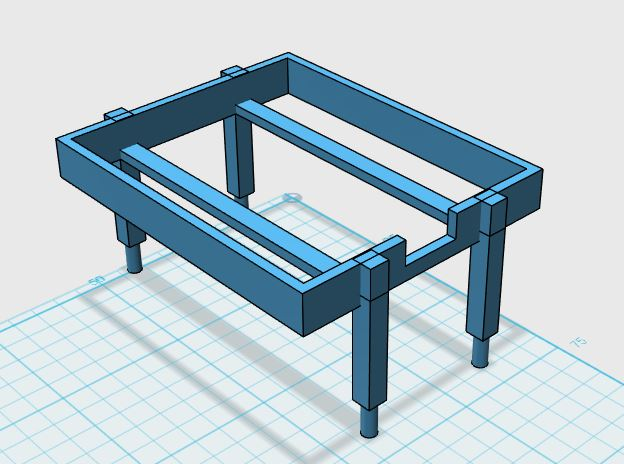
\includegraphics[width=0.4\linewidth]{images/BatteryHolder.JPG}
	}
	\subfloat[Pencil holder\label{fig:pencilHolder}]{
		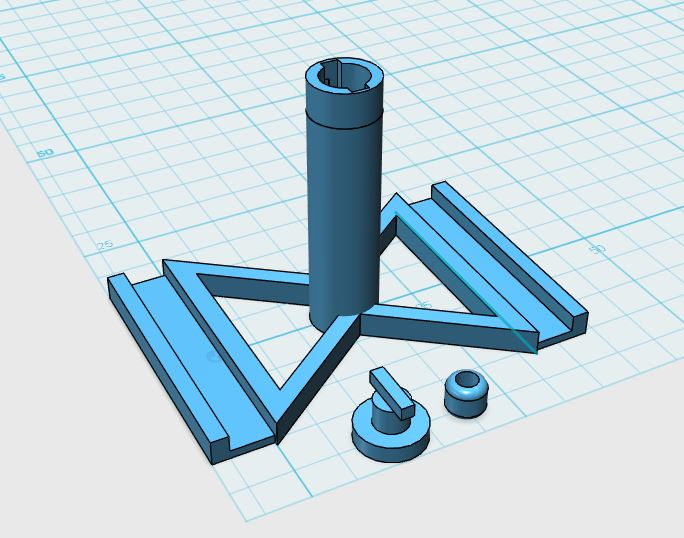
\includegraphics[width=0.4\linewidth]{images/PencilHolder.JPG}
	}\\
	\subfloat[Printed pencil holder\label{fig:pencilHolderReal}]{
		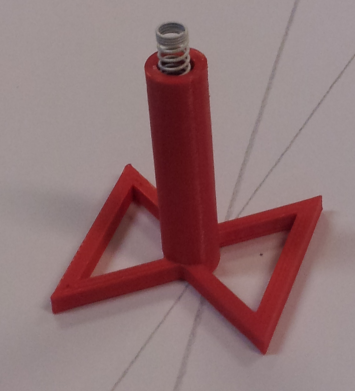
\includegraphics[width=0.4\linewidth]{images/penHolder.png}
	}
	\caption{3D printed utilities}
	\label{fig:3d}
\end{figure}
\begin{figure}[H]
	\centering
	\subfloat[Front of robot\label{fig:robotFront}]{
		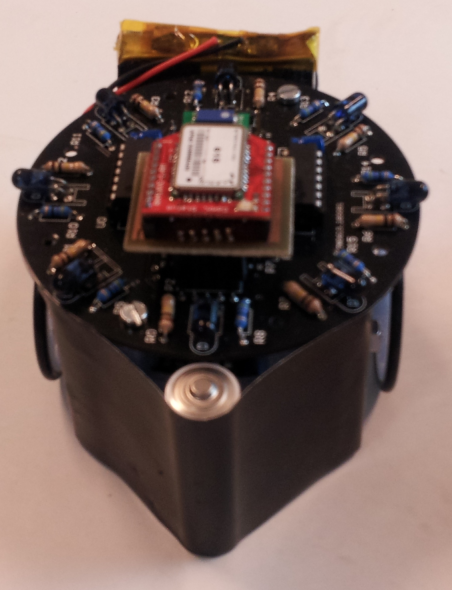
\includegraphics[width=0.4\linewidth]{images/robotFront.png}
	}
	\subfloat[Back of robot\label{fig:robotBack}]{
		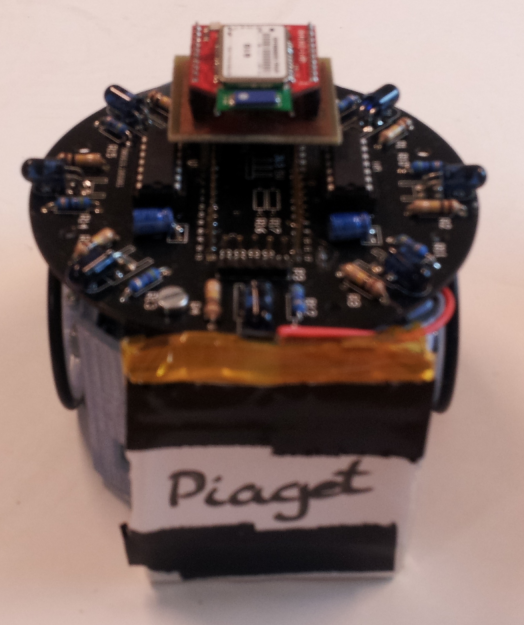
\includegraphics[width=0.4\linewidth]{images/robotBack.png}
	}\\
	\subfloat[Underside of robot\label{fig:robotUnder}]{
		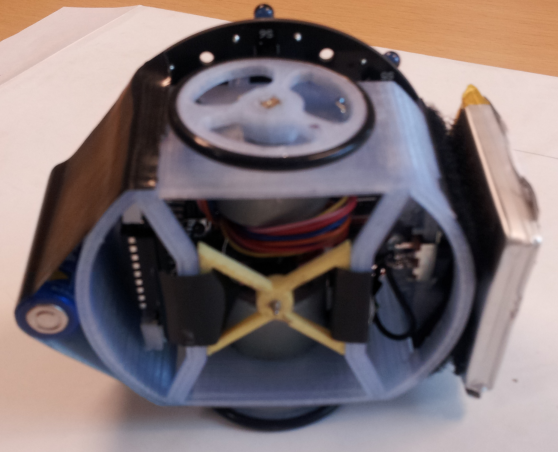
\includegraphics[width=0.4\linewidth]{images/robotUnder.png}
	}
	\subfloat[Robot drawing an angle\label{fig:robotDrawing}]{
		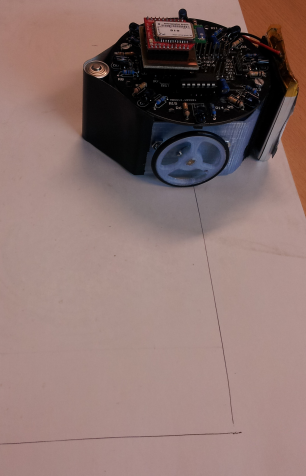
\includegraphics[width=0.4\linewidth]{images/robotDrawing.png}
	}
	\caption{Pictures of the robot}
	\label{fig:robot}
\end{figure}

\subsection{Bluetooth circuit board}
The \chirp team had previously tested using bluetooth communication between an android device and the robot. We therefore got help in creating the inital circuitry for our bluetooth module(figure~\ref{fig:circuitDrawing}). This drawing was at this point designed in the Eagle software in order to make it possible to produce at a later stage(~\ref{fig:circuitDesign}). 

\bigskip\noindent
The basic functionality of the circuit is to create a mapping between the receiver (\textbf{RX}) and transmission (\textbf{TX}) signals on the arduino and bluetooth module. In addition to the data signals the circuit board needed to map a 3.3V power supply (\textbf{VDD}) and a ground connection (\textbf{GND}) to the bluetooth module (see schematic in figure~\ref{fig:bluetoothSchematic}).

\image{images/schematicBluetooth2.PNG}{\linewidth}{Schematic of the bluetooth shield. Components on the right is the bluetooth module.}{fig:bluetoothSchematic}

\bigskip\noindent
As seen in figure~\ref{fig:bluetoothSchematic} we used a two components between the arduino TX signal and the bluetooth module RX (a 220$\Omega$ resistor and 3.3V zener diode). This was because the arduino operates on 5V, while the bluetooth module expected only 3.3V. Mapping these directly would most likely result in the destruction of the module. It should here be noted that the schematic does in show a normal diode, but the circuit is design for a zener diode and using a normal diode would not work.

\bigskip\noindent
It can be seen in figure~\ref{fig:circuitProto} that some soldering around the board was necessary on the prototype. The prototype did however lead us to conclude that the circuit itself was functional and we were able to proceed with creating all the circuit boards that we needed. 
Figure~\ref{fig:circuitTrans} shows the template used in the etching process when creating these boards. While figure~\ref{fig:circuitboard} shows the circuit board alongside with the bluetooth module we used for our robots. The complete assembly of the robot can be seen in figure~\ref{fig:robotDrawing}.

\begin{figure}[!htb]
	\centering
	\subfloat[Inital circuit\label{fig:circuitDrawing}]{
		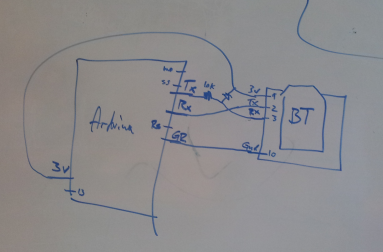
\includegraphics[width=0.4\linewidth]{images/bluetoothCircuit.png}
	}
	\subfloat[Created in circuit designer\label{fig:circuitDesign}]{
		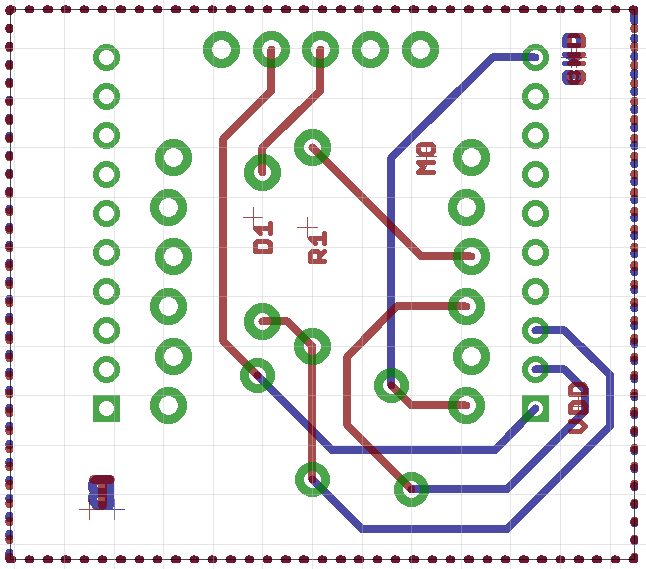
\includegraphics[width=0.4\linewidth]{images/circuitDrawing.PNG}
	}\\
	\subfloat[Prototype template\label{fig:circuitProtoTrans}]{
		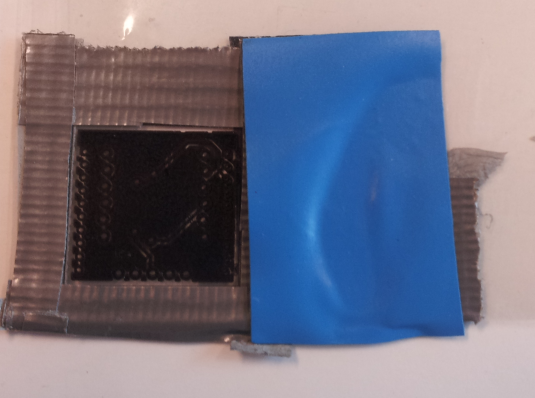
\includegraphics[width=0.4\linewidth]{images/bluetoothProtoTrans.png}
	}
	\subfloat[Prototype circuitboard\label{fig:circuitProto}]{
		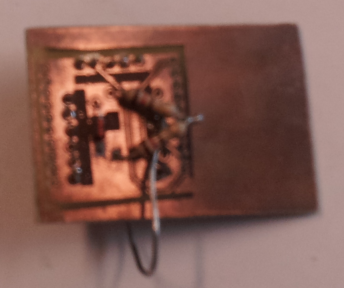
\includegraphics[width=0.4\linewidth]{images/bluetoothProto.png}
	}\\
	\subfloat[Finished template\label{fig:circuitTrans}]{
		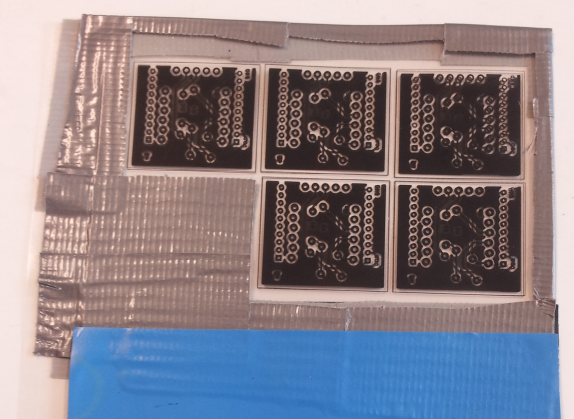
\includegraphics[width=0.4\linewidth]{images/bluetoothTrans.png}
	}
	\subfloat[Finished circuitboard\label{fig:circuitboard}]{
		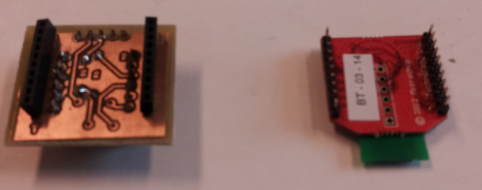
\includegraphics[width=0.4\linewidth]{images/bluetooth.png}
	}
	\caption{Circuit boards}
	\label{fig:circuit}
\end{figure}

\part{Results}
\chapter{Results}
In order to determine each students level of understanding and knowledge prior to the experiment, seven days before the first stession, a pretest was preformed using the test created in collaboration with the class' teacher~(Appendix~\ref{appendix:pretest}).

\bigskip\noindent
For the inital analysis of the data we used a independent-samples t-test.
This test is used to determine if a difference between the means in the two groups exists, and if this difference is statistically significant.
But in order to use this test the six assumption regarding study design and the nature of the data must first be confirmed to hold.

\bigskip\noindent
The first three assumptions are directed at how the study was designed.
The assumptions are; 
1) must have one dependent variable measured at the continous level, 2) must have one independent dichotomous variable, and 3) should have independence of observations. In our case all of these three assumptions hold. The dependent variable is \texttt{diff}, representing the diffrence from pretest to posttest, which is indeed a continous variable. The independent variable in this case is wether or not a participant were exposed to the robot or just the simulator, which we have encoded as \texttt{robot}. The last assumption as there was no overlap between the different group. It should however bit noted that participants from the different group could communicate with eachother when they were not actively participating the study(e.g. during the weekend, break, etc), but we do not see this as a major infraction of the assumption.

\bigskip\noindent
The last three assumption are directed at the nature of the data, and will require some extra analysis to verify. The forth assumption assumes that there should be no significant outliers in the different group in terms of the dependent variable. 

\image{images/results/boxplot.PNG}{\linewidth}{Boxplot of difference grouped by treatment}{fig:boxplot}

\bigskip\noindent
As seen in figure~\ref{fig:boxplot} an extreme outlier found found in our dataset within the robotics group(The asterix represents an extreme outlier in SPSS). By reassessing the tests, and investigating the circumstances during the pretest and posttest is was determined that the outlier result were must likely not caused by errors during assessment, data entry or the tests. As a result of this, a comparison of the results with and without the outlier was conducted (see table~\ref{table:outliers}). It should be noted that the results without the outliers failed Levene's test for equality of variances ($p = 0.033$) and results in the table are therefore produced by using the Welch t-test. Both do however show that there was no statistically significant difference in mean difference score between the robotics and simulator group($p > 0.05$ for both results). 

\bigskip\noindent
\smalltable{Comparasion of results with and without outliers, using independent samples t-test}{table:outliers}{
	\begin{tabular}{llllll}\hline
		Include outliers & t & df & Sig. & Mean difference & Std. Error difference\\\hline
		No & 0.232 & 7.05 & 0.823 & 0.25 & 1.078\\
		Yes & 0.967 & 9 & 0.359 & 1.6 & 1.655\\\hline
	\end{tabular}
}


\bigskip\noindent
\smalltable{Tests means for different groups}{table:means}{
	\begin{tabular}{lll}
		Group & Pretest mean & Posttest Mean\\\hline
		Robot & 18.40 & 18.80\\
		Simulator & 13.17 & 15.17\\
		All & 15.54 & 16.82\\\hline
	\end{tabular}
}
\smalltable{Paired samples T-test of differences}{table:paired}{
	\begin{tabular}{lllllll}\hline	
		Group & \multicolumn{3}{l}{Paired differences} & t & df & Sig.(2-tailed)\\
		\cline{2-4}
		& Mean & Std deviation & Std. error mean & & &\\\hline
		Robot & 0.40 & 3.13 & 1.40 & 0.29 & 4 & 0.79\\
		Simulator & 2.00 & 2.37 & 0.97 & 2.07 & 5 & 0.09\\\hline
	\end{tabular}
}
\smalltable{Indenpendent Samples T-test of differences, group by pretest-score}{table:score}{
	\begin{tabular}{lllll}\hline
		Group & N & Difference mean & Std. Deviation & Std. Error Mean\\\hline
		$Score >= 15$ & 6 & 0.33 & 2.80 & 1.15\\
		$Score < 15$ & 5 & 2.44 & 2.41 & 1.08\\\hline
	\end{tabular}
}
\smalltable{Tests of Normality}{table:normality}{
	\begin{tabular}{l|lll|lll}\hline
		Group & \multicolumn{3}{l}{Kolmogorov-Smirnov} & \multicolumn{3}{l}{Shapiro-Wilk}\\\cline{2-4}\cline{5-7}
		& Statistic & df & Sig. & Statistic & df & Sig.\\\hline
		Robot & 0.376 & 5 & 0.020 & 0.788 & 5 & 0.065\\
		Simulator & 0.164 & 6 & 0.200 & 0.950 & 6 & 0.739\\
		All & 0.187 & 11 & 0.200 & 0.927 & 11 & 0.380\\\hline
	\end{tabular}
}
\part{Discussion}
\chapter{Discussion}

\part{Conclusion}
\section{Conclusion}
During this project we have constructed an initial setup for IDI in educational robotics. 
We had performed a literature review to find the state of the art of educational robotics in the field of mathematics. 
We have also given an introduction to the pedagogical aspects, and the research methodologies needed when conducting such research.
We created a test to measure knowledge in the area of angle estimation, calculation and understanding. (The test was found to be reliable and valid. )`?
We have created chassis extensions for the robot and a bluetooth module platform which can be used for several other components as well.

We have investigated how a robot can be used to teach mathematics to school students. We have also found strengths and weaknesses of using a robot compared to a simulator. 

We have established a relationship between IDI and the international school in Trondheim which can help other researchers when expanding on our project. In addition our project serves as an introduction in itself for researchers wanting to look into educational robotics. 

The robotic activities did help students content knowledge about angles, and did aid in their understanding and ability to explain what an angle is. However the difference from a simulator was not statistically significant.


\clearpage
\bibliographystyle{plain}
\bibliography{refs}

\begin{appendices}
	%\chapter{Algorithms}
	%\begin{algorithm}
	\caption{Boilerplate}%\label{alg:euclid}
	\begin{algorithmic}[1]
		\Procedure{Boilerplate}{}
			\State \textbf{return} $4$\Comment{Random number decided by fair diceroll}
		\EndProcedure
	\end{algorithmic}
\end{algorithm}
	%\begin{algorithm}
	\caption{Euclids algorithms}\label{alg:euclid}
	\begin{algorithmic}[1]
		\Procedure{Euclid}{$a,b$}\Comment{The g.c.d of a and b}
			\State $r\gets a\bmod b$
			\While{$r\not=0$}\Comment{We have the answer if r is 0}
				\State $a\gets b$
				\State $b\gets r$
				\State $r\gets a\bmod b$
			\EndWhile\label{alg:euclid:endwhile}
			\State \textbf{return} $b$\Comment{The gcd is b}
		\EndProcedure
	\end{algorithmic}
\end{algorithm}
	\begin{algorithm}
	\caption{ID3}\label{alg:id3}
	\begin{algorithmic}[1]
		\Procedure{ID3}{$D$,$Attributes$,$Target$}
			\State $t\gets createNode()$
			\If{$\forall\langle x,c(x)\rangle \in D: c(x) = 1$}
				\State $t.label\gets 1$
				\State \textbf{return} $t$
			\ElsIf{$\forall\langle x,c(x)\rangle \in D: c(x) = 0$}
				\State $t.label\gets 0$
				\State \textbf{return} $t$
			\ElsIf{$Attributes = \emptyset$}
				\State $t.label\gets mostCommonClass(D, Target)$
				\State \textbf{return} $t$
			\Else
				\State $A^* = \argmax{A\in Attributes}IG(D, A)$
				\ForAll{$a\in A^*$}
					\State $D_a\gets\{(x,c(x))\in D : x\|_{A^*}=a\}$
					\If{$D_a = \emptyset$}
						\State $t'\gets createNode()$
						\State $t'.label = mostCommonClass(D, Target)$
						\State $createEdge(t, a, t')$
					\Else
						\State $createEdge(t, a, ID3(D_a, Attribute -\{A^*\}, Target))$
					\EndIf
				\EndFor
			\EndIf
			\State \textbf{return} $t$
		\EndProcedure
	\end{algorithmic}
\end{algorithm}
	\begin{algorithm}
	\caption{Basic K-means algorithm}\label{alg:kmeans}
	\begin{algorithmic}[1]
		%\Procedure{K-means}{K}
			\State Select $K$ points as inital centroids.
			\Repeat
				\State Form $K$ clusters by assigning each point to its closest centroid.
				\State Recompute the centroid of each cluster
			\Until Centroids do not change
		%\EndProcedure
	\end{algorithmic}
\end{algorithm}
	\begin{algorithm}
	\caption{Basic agglomerative hierarchical clustering algorihms.}\label{alg:agglomerative}
	\begin{algorithmic}[1]
			\State Compute the proximity matrix, if necessary.
			\Repeat
				\State Merge the closest two clusters.
				\State Update the proximity matrix to replect the proximity between the new cluster and the original clusters.
			\Until Only one cluster remains.
	\end{algorithmic}
\end{algorithm}
	\begin{algorithm}
	\caption{DBSCAN algorithms}\label{alg:dbscan}
	\begin{algorithmic}[1]
		\State Label all the point as core, border, or noise points.
		\State Eliminate noise points.
		\State Put an edge between all core points that are within $Eps$ of each other.
		\State Make each group of connected core points into a separate cluster.
		\State Assign each border point to one of the clusters of its associated core points.
	\end{algorithmic}
\end{algorithm}
		
\end{appendices}

\end{document}

